%% Template para dissertao/tese na classe thesisdifctunl  
%%  EM  DESENVOLVIMENTO - Dezembro de 2007
%%
%% Carrega a classe thesisdifctunlpt
%% Opes: 
%% * Idiomas
%%           pt   - portugus 
%%           en   - ingls
%% * Tipo de texto
%%           lei  - licenciatura
%%           premei - preparao de dissertao
%%           mei  - mestrado
%%           prop - proposta de doutoramento
%%           prephd - preparao de tese
%%           phd  - doutoramento
%%   * Tipo de impresso
%%            print
%%    * Pginas
%%           oneside - para impresso em face nica
%%           twoside - para impresso em frente e verso
\documentclass[pt, premei, twoside, print]{thesisdifctunl}

%% Prembulo:
%% coloque aqui o seu prembulo LaTeX, i.e., declarao de pacotes,
%% (re)definies de macros, medidas, etc.
\usepackage{tweaklist}
\usepackage{setspace}
\usepackage{multirow}
\setcounter{tocdepth}{4}
%% Identificao:
% Universidade
\university{Universidade Nova de Lisboa}
% Endereo (cidade).
\address{Lisboa}
% Faculdade
\faculty{Faculdade de Ci�ncias e Tecnologia}
% Departamento 
\department{Departamento de Inform�tica}
% Curso
\program{Mestrado em Engenharia Inform�tica}
% rea cientfica
\majorfield{Engenharia Inform�tica}
% Ttulo da dissertao/tese
\title{Secure and reliable routing for dependable wireless sensor networks}

% Data 
\date{1� Semestre de 2009/10 \\ \smallskip
5 de Fevereiro de 2010}

% Autor
\author{Pedro Miguel Oliveira Marques da Silva (n� 26649)}

% Orientador(a)
% Opo: [f] - para orientador do sexo feminino
\adviser[m]{Prof. Doutor Henrique Jo�o Lopes Domingos}

% Co-orientador(a)
%\coadviser{Prof. Doutor nome do co-orientador}

%% Inicio do documento
\begin{document}
\onehalfspacing
%% Parte pr-textual
\frontmatter

% Folha de rosto. Comente para ocultar
\frontpage

% Pgina de apresentao. Comente para ocultar
\presentationpage

% Agradecimentos. Se preferir, crie um ficheiro  parte e inclua com \include{}
%\acknowledgements
% O texto ...

% Resumo em Portugus
% Se preferir, crie um ficheiro  parte e inclua com \include{}
\resumo
As redes de sensores s�o uma tecnologia emergente no dom�nio da monitoriza��o, de forma aut�noma, de
ambientes fisicos. S�o formadas por pequenos dispositivos que se auto-organizam por modo a cobrirem
uma �rea geogr�fica, podendo formar uma rede de larga escala com milhares de n�s. Esta autonomia e
auto-organiza��o apresenta alguns desafios relacionados com os aspectos de seguran�a, nomeadamente,
no que concerne com o encaminhamento de dados. O trabalho a realizar pretende contribuir para a
cria��o de um modelo sist�mico para o estudo de protocolos de encaminhamento seguro em
redes de sensores sem fios (RSSF). A defini��o do modelo de advers�rio � o passo
inicial para o enquadramento das tipologias de ataque que se pretende avaliar.
Aliado ao modelo formal de Dolev-Yao, orientado para os ataques ao meio de
comunica��o, o estudo de novos modelos de advers�rio, relacionados com a
intrus�o e captura de n�s � pertinente e apresentado dentro do �mbito deste trabalho.

Com vista a tornar as RSSF resistentes a algumas tipologias de ataques
preconizadas no modelo de advers�rio, t�m vindo a ser desenvolvidos diversos
algoritmos de encaminhamento seguros. Pretende-se estudar alguns destes
algoritmos, representantes do estado da arte neste dom�nio, estabelecendo uma
matriz de medidas de resist�ncia ao modelo de advers�rio, que permita ent�o avaliar a efectividade
destes .

Como contributo principal deste trabalho destaca-se a concep��o de um ambiente de simula��o
inovador, uma vez que se pretende implementar funcionalidades n�o encontradas nos sistemas de
simula��o para as RSSF existentes. Este sistema proporcionar� a possibilidade de desenhar e avaliar
algoritmos de encaminhamento, concebidos para serem seguros, quando sujeito a ataques definidos no
modelo de advers�rio. Este avalia��o estar� centrada fundamentalmente na an�lise propriedades como o
consumo de energia, fiabilidade, lat�ncia, correc��o dos dados e correc��o do comportamento do
potocolo.
% Palavras-chave do resumo em Portugu�s
\begin{keywords}
Redes de sensores sem fios,Protocolos de encaminhamento seguros,Simula��o
de redes de sensores, Ataque por intrus�o
\end{keywords}
% to add an extra black line
~\\ ~\\\rule{\textwidth}{0.2mm}




% Resumo em Ingls
% Se preferir, crie um ficheiro  parte e inclua com \include{}
\abstract
Wireless Sensor Networks (WSN) are an emerging and very interesting technology applied to 
different applications. They are formed by small, self organized devices that cooperate to
form a large scale network with thousands of nodes covering a large area.
The independent operation of the devices and the self-organization feature of the network present
some challenges related to security, particularly regarding the security of the processed and routed
data over the network.  

This work aims to contribute to the study of the security conditions
and robustness criteria of routing protocols  for WSN. This study must be performed from a
systemic model of assessement and from an experimental comparison of
protocols, based upon a simulation platform which will enable to assess their operation in
closed-to-real operating conditions.  The simulation platform will be equipped with the needed tools
and components, in order to enable experimental evaluation of secure and intrusion tolerant
protocol. These protocols combine mechanisms and defensive counter-measures against
attacks on communications, inspired by the Dolev-Yao adversary model. They include also mechanisms
to prevent specific routing attacks, which can be triggered from the injection or from the
replication of misbehavior of operation, in nodes that have been subjected to intrusion attacks. 

The major contribution of this work is the design of an innovative simulation environment, since
some of its features are not found in existing WSN simulation systems. It will provide the
opportunity to implement and evaluate routing
algorithms that are designed to be secure but for which there are no
experimental studies on the real robustness and impact of designed
security mechanisms. This evaluation will focus primarily on examining the effectiveness of the
provided
security mechanisms. Additionally, it will also assess the
impact of these mechanisms in relation to energy consumption, reliability, latency and resistance of
the protocol, regarding the coverage and the scale of the network.
~\\ ~\\ \rule{\textwidth}{0.2mm}


% ndice. 
\tableofcontents

% Lista de figuras. Comente para ocultar
\listoffigures

% Lista de tabelas. Comente para ocultar
\listoftables

%% O contedo principal
\mainmatter

%  aconselhvel ter um captulo por ficheiro :
% "capitulo1.tex", "capitulo2.tex", ... "capituloN.tex" e depois
% inclu-los com:
\chapter{Introdu��o} \label{cap:introducao}
\onehalfspacing
\section{Introdu��o geral} \label{sect:introducao}
Recentemente, t�m-se observado avan�os na concep��o e fabrico de sistemas computacionais
program�veis, baseados em \textit{hardware} de pequena dimens�o, \cite{MEMS} com capacidade para
desempenhar tarefas espec�ficas. Estes avan�os permitiram integrar, nesses sistemas, processadores
miniaturizados, mem�ria, dispositivos de processamento de sinal e de convers�o anal�gica-digital
para a detec��o de diferentes fen�menos f�sicos (atrav�s de diversos tipos de sensores) e
capacidades de comunica��o sem fios por r�dio frequ�ncia (com base nas normas 802.15.4 
\cite{ietf_802154,zigbee_802154} e Zigbee \cite{zigbee_802154})). A possibilidade de constru��o
destes dispositivos (que se designam mais simplesmente por n�s sensores) fez surgir, nos �ltimos
anos, um novo campo da investiga��o conhecido por redes de sensores sem fios (RSSF).

Uma RSSF � formada por um conjunto de dispositivos com as caracter�sticas descritas anteriormente,
distribu�dos numa certa �rea geogr�fica, que podem funcionar de forma aut�noma ou sem supervis�o
humana. Estas redes permitem monitorizar, com maior ou menor densidade, diferentes fen�menos f�sicos
associados ao meio ambiente envolvente. As RSSF possuem caracter�sticas de auto-organiza��o, podendo
ser formadas por um menor ou maior n�mero de sensores, permitindo cobrir desde pequenas a vastas
�reas de monitoriza��o. Um ambiente de instala��o de uma rede pode ser um edif�cio, uma instala��o
industrial, uma �rea de combate, uma vasta zona de monitoriza��o de um habitat natural, um ve�culo
ou o pr�prio corpo humano \cite{apps_tracking,app_monitor,app_health,Akyildiz2002}.

A componente b�sica e fundamental de uma rede de sensores �, pois, o n� sensor (tamb�m designado por
\textit{mote}) \cite{mica2_datasheet, btnodes,sunspotworld,micaz}. Cada um destes n�s constitui um
substrato computorizado que pode possuir diversos sensores para monitorizar, por exemplo,
temperatura, luz, movimento e outros fen�menos f�sicos, consoante as necessidades das aplica��es.
Sendo um dispositivo miniaturizado e concebido para possuir um baixo custo de produ��o, apresenta um
poder de computa��o limitado, baixa largura de banda de comunica��o, curto alcance de comunica��o
r�dio e energia aut�noma limitada (com base em baterias do tipo AAA ou de c�lulas fotovoltaicas) 
\cite{Yick2008}. Numa RSSF a energia pode constituir um recurso finito. Em certos ambientes de
instala��o pode n�o ser poss�vel, ou vi�vel, realizar opera��es que exijam interven��o ou supervis�o
humana, por exemplo, para o carregamento ou substitui��o de baterias. Em certos ambientes de
instala��o pode n�o ser poss�vel, ou vi�vel, realizar opera��es que exijam interven��o ou supervis�o
humana, por exemplo, para o carregamento ou substitui��o de baterias. Conhecidas estas limita��es,
para se poderem atingir distribui��es de grande cobertura geogr�fica, os sensores t�m de ser
distribu�dos em grande n�mero, podendo-se tamb�m, por esse meio, aumentar a redund�ncia dos n�s que,
assim, formam redes de larga escala que chegam a atingir milhares de n�s.

Os \textit{motes} podem diferir uns dos outros consoante a sua fun��o na rede e poder�o desempenhar,
fundamentalmente, dois papeis: n� gen�rico gerador de informa��o (\textit{source-nodes}) e n� base
ou de sincroniza��o (n� colector de dados da rede ou de execu��o de comandos de pesquisa). Numa RSSF
os n�s podem tamb�m actuar como n�s de interliga��o (ou de encaminhamento e processamento interm�dio
atrav�s da rede) ou \textit{gateways } (que permitem ligar o ambiente da rede de sensores a outras
redes e sub-sistemas externos). Uma RSSF pode ser concebida de forma a ser interligada a outras
infraestruturas computacionais que, com maior capacidade de armazenamento e processamento, permitem
efectuar an�lise de dados coligidos. Na tecnologia actual existem ainda n�s de desenvolvimento, que
possuem liga��es a computadores (ex: liga��o de rede \textit{Ethernet}, RS-232 ou USB), permitindo o
carregamento expedito de c�digo desenvolvido em esta��es de desenvolvimento. Os
sensores dotados de liga��es Ethernet, RS-232 ou USB podem ainda funcionar como n�s de tipo
\textit{gateway},
permitindo, num cen�rio concreto, ligar a rede de sensores a aplica��es, executando em sistemas de
computadores usuais \cite{gateways}.
\subsection{Caracteriza��o de RSSF}\label{sect:subsec_caracterizacao_wsn}
As redes de sensores sem fios podem ser abordadas como um caso especial de redes \textit{ad-hoc},
embora exibam caracter�sticas espec�ficas \cite{Corson1999}. As RSSF para aplica��es de larga escala
fazem emergir algumas problem�ticas inerentes a aplica��es distribu�das, com especificidades e
desafios pr�prios \cite{Coulouris_sd4ed}, nomeadamente ao n�vel dos mecanismos de gest�o, da
organiza��o topol�gica aut�noma, das necessidades de sistemas de encaminhamento\textit{ multi-hop},
de requisitos de toler�ncia a falhas, de requisitos de escalabilidade ou de necessidade de servi�os
de seguran�a. 
\subsection{Aplica��es}
Muitas foram as aplica��es \cite{Akyildiz2002,Kuorilehto2005} encontradas na investiga��o ou na
utiliza��o emergente de RSSF com diferentes requisitos de escala \cite{Yick2008}. O car�cter
aut�nomo destas redes oferece um sem n�mero de vantagens que propicia a sua utiliza��o em locais
remotos de acessibilidade dif�cil e onde n�o � poss�vel a sua manuten��o e supervis�o. De entre as
aplica��es das RSSF, podem destacar-se as seguintes: 
\begin{descriptionNoIndent}
 \item \textbf{Detec��o de alvos/objectos(\textit{Target Tracking}):}  \cite{apps_tracking}
associada � detec��o de movimento (traject�ria/presen�a) em �reas vigiadas (como, por exemplo, em
teatros operacionais militares ou na vigil�ncia e monitoriza��o de recursos ou infraestruturas);
 \item \textbf{Monitoriza��o de fen�menos naturais:}  \cite{app_monitor}
associada � detec��o de eventos ou anomalias ambientais (com aplica��es na agricultura,
monitoriza��o de polui��o ou monitoriza��o de habitats naturais), bem como de vigil�ncia ou controlo
de fen�menos naturais (sismos, actividade de vulc�es, etc);
 \item \textbf{Recolha de dados:} \cite{app_health} associada ao controlo de indicadores f�sicos ou
biom�dicos de pessoas ou de animais (com recurso a sensores especiais, associados a aplica��es da
medicina) ou como ambientes de monitoriza��o de opera��o de infraestruturas cr�ticas (pontes,
edif�cios, sistemas electromec�nicos ou equipamentos de instala��es fabris). 
\end{descriptionNoIndent}
\section{Seguran�a em RSSF} \label{sect:seguranca_rssf}
A seguran�a nas RSSF �, \textit{de facto}, um problema, quando se perspectiva a sua utiliza��o para
sistemas cr�ticos. A seguran�a deve ser pensada em tempo de concep��o \cite{Perriga}, tendo em
vista a abrang�ncia do sistema e tendo em aten��o as particularidades espec�ficas da tecnologia
inerente, bem como dos ambientes onde s�o implementadas. Importa analisar as hip�teses de
desencadeamento de ataques a estas redes (a partir da defini��o de modelos de advers�rio) bem como
as repercuss�es das potenciais tipologias de ataques que representem o modelo de
advers�rio \cite{Attaks_defenses_sec_in_wsn,Karlof2003}. Esta an�lise deve ser feita tendo em conta
a pilha de protocolos \cite{Akyildiz2002} e de servi�os
associados ao \textit{software} \cite{tinyos,contiki,Karlof2004,SPINS} que executa em cada n�, uma
vez que cada uma das camadas de servi�os e protocolos pode ser vulner�vel a esses ataques. 

Na abordagem de uma plataforma usual e gen�rica para um n� de uma RSSF, verifica-se que, em geral,
cada n� apresenta uma pilha minimalista de protocolos e servi�os, por compara��o com uma pilha
associada a uma rede de computadores usual (ex., TCP/IP ou pilha OSI) \cite{sd_tanenbaum}. As
limita��es impostas pelas dimens�es e as capacidades de opera��o n�o permitem uma arquitectura muito
ambiciosa e, por outro lado, as RSSF possuem geralmente uma voca��o orientada para aplica��es
espec�ficas, que condicionam os servi�os que devem ser suportados na pilha. As camadas de opera��o
de um n� sensor s�o essencialmente cinco \cite{Akyildiz2002}: camada f�sica, camada de liga��o de
dados, camada de rede, camada de transporte e camada de aplica��o. Todavia, na maior parte dos
casos, a camada de transporte de dados e a funcionalidade inerente � camada de rede s�o concebidas
de forma mais ou menos espec�fica, tendo em vista as caracter�sticas particulares das aplica��es. Na
investiga��o, verifica-se ainda que a camada de liga��o de dados (n�vel MAC e protocolos data-link)
foram objecto de v�rias propostas, com diferentes variantes que podem apresentar vantagens
particulares, dados os requisitos de opera��o das aplica��es \cite{BMAC,SMAC,mac_protocols}.
\begin{figure}[ht]
\centering
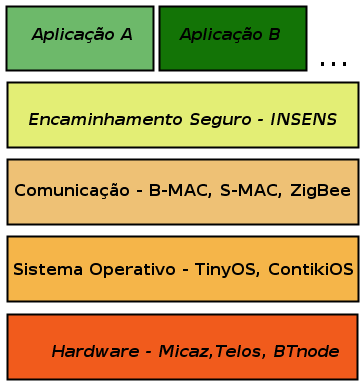
\includegraphics[height=4cm,width=3cm]{pilha_soft.png}
\caption{Pilha de Servi�os de uma RSSF} \label{fig:stack_serv}
\end{figure}
Alguns autores \cite{SIGF,INSENS,clean_slate} t�m vindo a desenhar algoritmos com vista a minimizar
o impacte dos ataques ao encaminhamento, durante a opera��o das RSSF. Estes algoritmos pretendem
garantir algumas propriedades b�sicas de seguran�a \cite{perrig_design_sec_sensor} (ex:
confidencialidade, integridade, autentica��o, detec��o de retransmiss�o il�cita de dados). N�o
obstante, devem ser consideradas outras tipologias de ataques especificamente associados ao suporte
de encaminhamento de dados na rede. Diferentes protocolos de encaminhamento seguro em RSSF endere�am
apenas algumas dessas tipologias mas, em geral, n�o contemplam contra-medidas globais face a todas.
Por outro lado, muitas das propostas apresentadas t�m por base modelos matem�ticos, an�lises
te�ricas ou experi�ncias de pequena dimens�o. Torna-se importante que esse estudo te�rico seja
complementado e verificado, tendo em conta o desempenho desses protocolos com an�lises experimentais
mais pr�ximas dos ambientes reais em que a rede opera. Para tal, o recurso a ambientes de simula��o
torna-se uma direc��o importante de apoio a este estudo.
\section{Objectivos e contribui��es previstas para a disserta��o} \label{sect:solucao}
Uma das vertentes do estudo da seguran�a em RSSF tem que ver com a possibilidade de se poderem
efectivar ataques ao n�vel do encaminhamento de dados (da pilha de suporte de servi�os de
\textit{software}, \figurename{ \ref{fig:stack_serv}}). Diferentes tipologias de ataques 
\cite{Karlof2003,Hu2004,Perriga} exigem diferentes tipos de contra-medidas. Estas, normalmente, s�o
combinadas em mecanismos de seguran�a, consoante as propostas de sistemas de encaminhamento seguro.
Estes s�o implementados tendo em conta as caracter�sticas e o modo de opera��o das RSSF
\cite{SPINS,Luk2007d,Karlof2004}. 

Conhecidas que est�o as dificuldades existentes no estudo de protocolos de encaminhamento
seguro \cite{Karlof2003,Sec_WSN_Vulnerabilities}, estes permanecem como um dos aspectos em aberto e
como um desafio � concep��o de RSSF que operem em condi��es de seguran�a. Este desafio � tanto mais
relevante quanto a an�lise de seguran�a pode envolver a avalia��o de diferentes modelos e hip�teses
de advers�rio \cite{Dolev1983,Parno2005} e tipologias de
ataques \cite{Attaks_defenses_sec_in_wsn,Karlof2003}. Estas tipologias nem sempre s�o estudadas de
forma sistem�tica e comparativa, na abordagem de diferentes protocolos de encaminhamento seguro que
v�o sendo propostos. Por outro lado, existe uma dificuldade adicional em poder conjugar-se o estudo
das contra-medidas de seguran�a importantes com a sua avalia��o experimental face � implementa��o.
Para cada protocolo interessa medir o impacte que diferentes tipologias de ataques podem
ter, nomeadamente, em cen�rios de grande escala, o que exige a utiliza��o de sistemas de simula��o
\cite{ns2,jsim,SENSE,shox,jprowler,freemote} de RSSF que permitam simular diferentes hip�teses de
ataque e antecipar o seu impacte. Este impacte deve ser analisado n�o apenas no que refere ao
comportamento dos protocolos mas, complementarmente, no que refere � forma como afectam a pr�pria
rede nomeadamente, em termos de consumo de energia, fiabilidade e lat�ncia. Um sistema que suprima
estas dificuldades contribui para um mais r�pido desenvolvimento e uma afina��o mais cuidada de
determinados par�metros dos protocolos, com vista a garantir as propriedades de seguran�a desejadas
para o ambiente de opera��o das RSSF, em condi��es mais realistas.

No �mbito do trabalho que se pretende desenvolver na elabora��o da disserta��o, ir� ser concebido e
desenvolvido um sistema de simula��o inovador. Este sistema dever� permitir o estudo sistem�tico de
protocolos de encaminhamento, desenhados para serem seguros, e dever� possuir, em particular, as
seguintes funcionalidades: 
\begin{itemize}
\item Interface de visualiza��o e configura��o da rede com informa��es dos par�metros de simula��o e
informa��o de cada n� (por exemplo, o seu estado energ�tico); 
\item Implementa��o de um modelo de energia que permita extrair consumos em diferentes momentos de
opera��o: opera��o normal e opera��o perante determinado ataque; 
\item Modelo parametriz�vel de gera��o de topologias, podendo estas ser definidas como: distribui��o
aleat�ria, distribui��o em grelha, distribui��o controlada (estruturada); 
\item Mecanismo de introdu��o de falhas/ataques na rede. Com este mecanismo pretende-se permitir o
estudo do comportamento dos protocolos face � possibilidade de introduzir ataques tipificados; 
\item Utilit�rios de recolha de dados da simula��o, em tempo real e em tempo diferido, que permitam
a extrac��o de medi��es referentes a propriedades importantes, como consumos de energia, lat�ncia,
fiabilidade, correc��o do protocolo e correc��o dos eventos, disponibilizando-os de forma gr�fica. 
\end{itemize}
O ambiente de simula��o em causa permitir� estudar, sistem�tica e comparativamente, diferentes
protocolos de encaminhamento seguro em RSSF. Contribuir�, ainda, com o estabelecimento de uma base
de compara��o, pelo desenvolvimento de dois protocolos, para futuras avalia��es de outros protocolos
emergentes. Esta avalia��o ser� referente ao impacte que os mecanismos de seguran�a t�m sobre
propriedades t�o importantes como: o consumo de energia, a fiabilidade da rede, a lat�ncia das
comunica��es, correc��o dos dados e a correc��o do protocolo. Estas propriedades s�o,
normalmente,extrapoladas da implementa��o experimental em pequena escala ou da adop��o de modelos
matem�ticos, os quais, devido a vari�veis externas, pr�prias do ambiente de opera��o, se podem 
afastar bastante dos resultados reais.
\chapter{Trabalho relacionado} \label{cap:trabrelacionado}

Compete, neste cap��tulo, explanar o estado da arte em cada uma das
vertentes do trabalho, por forma a sustentar a discuss�o da adequabilidade da
solu��o proposta. Sabendo que a componente de an�lise cr�tica � de indispens�vel
presen�a num trabalho cient�fico, procurar-se-�, sempre que oportuno, acompanhar
as explica��es com uma interpreta��o t�cnica, como forma de justificar as
op��es efectuadas face  pan�plia de alternativas existentes na academia.
\section{Desenho e Implementa��o de RSSF Seguras }
\label{sect:sec_secure_wsn_design}
Sendo o tema central do trabalho proposto o estudo das propriedades de
seguran�a nestas redes, importa, em primeiro lugar, perceber, de forma
consistente, a sua arquitectura de protocolos. Em segundo lugar, � necess�rio
entender quais os servi�os de seguran�a disponibilizados, por forma a
poder adequar-se �s aplica��es para as quais s�o criadas
e desenhadas as RSSF.
\subsection{Arquitectura de uma RSSF}
\label{sect:subsec_arq_sofware_wsn}
As redes de sensores t�m uma arquitectura considerada minimalista porque, ao
contr�rio de outras arquitecturas de redes, est�o organizadas em menos camadas,
fundindo algumas fun��es desempenhada por camadas inferiores para outras
superiores ( ex: a camada de aplica��o pode desempenhar algumas fun��es da
normalmente atribu�das � camada de transporte). Assim, � fundamental perceber
qual a pilha de protocolos que as RSSF implementam, bem como perceber quais os
sistemas que comp�em um sensor gen�rico para de seguida apresentar algumas
implementa��es de sensores.
\subsubsection{Modelo da plataforma gen�rica de uma RSSF - \textit{Mote}}
� semelhan�a do que acontece com as redes convencionais, existem n�s de
computa��o interligados por uma infraestrutura de comunica��o. No caso da RSSF,
esta infraestrutura corresponde a comunica��o \textit{multi-hop} em que cada n�
da rede (\textit{mote}) pode desempenhar pelo menos tr�s papeis: 1) N� gerador
de dados, pela capta��o da eventos associados �s especificidades dos sensores
possu�dos; 2) N� encaminhador, que recebe dados de outros n�s e os passa a
outros n�s por forma a que alcance o destino; 3) N� de sincroniza��o ou n� de
agrega��o, embora estas duas caracteriza��es n�o correspondam � mesma tarefa
por si s�, a um n�vel mais macro, corresponde igualmente a colec��o de dados da
rede oriundos da detec��o de eventos, por forma a faze-la seguir agregada para
outro destino (interno ou externo � rede ).

Desta forma interessa perceber qual o modelo inerente a estas pequenas
plataformas de rede que apesar das caracter�sticas limitadoras da sua execu��o
conseguem executar uma complexidade de aplica��es tendo em conta sempre as
limita��es impostas pela arquitectura. Na figura seguinte apresent-se um
modelo \cite{ MODELO_SENSOR} que ilustra os diversos componentes que concorrem
para a efectividade de servi�o de um \textit{mote} numa RSSF.
\input{pic_sensornode}
Como se pode observar pela figura, da qual se pode generalizar o modelo de uma
plataforma gen�rica de RSSF, os sistemas que est�o presentes s�o os seguintes:
i) Sistema de processamento;ii) Sistema de energia; iii) Sistema de
comunica��o; iv) Sistema sensorial; v) Sistema de mem�ria.
\subsubsection{Arquitectura de \textit{Software} }
Uma das vis�es estruturais da uma RSSF, � a que apresenta pelas camadas de \textit{software} que a
comp�e. Esta vis�o permite ver a plataforma sobre a forma de um conjunto de servi�os que
desempenham tarefas especificas e que lhes permite em cada camada adequar os mecanismos intrinsicos
ao funcionamento, observe-se a figura seguinte que representa esta arquitectura, comparada com o
modelo tradicional das redes 802.2.

\subsubsection{Pilha de Protocolos de uma RSSF }
Uma arquitectura para a a pilha de protocolos em RSSF foi proposta por
\cite{Akyildiz2002}, esta pilha apresenta-se representada por cinco camadas:
\paragraph*{Camada F�sica.}� respons�vel por selec��o de frequ�ncia, detec��o de sinal e modula��o
tendo a minimiza��o do consumo de energia como uma prioridade;
\paragraph*{Camada de Liga��o de Dados.} Das tarefas associadas a estacamada destacam-se as
seguintes: multiplexa��o de dados, acesso ao meio, detec��o de erros/colis�es e detec��o de frames.
Uma RSSF pode ter um protocolo de MAC espec�fico(ex: B-MAC\cite{BMAC}, S-MAC \cite{SMAC}) de modo
agerir o consumo de energia consoante aos protocolos das camadas superiores;
\paragraph*{ Camada de Rede.} sendo a energia um tema transversal a toda a pilha,
esta camada deve endere�ar esta preocupa��o tamb�m, tem como tarefa prim�ria decidir quais os n�s a
escolher para o encaminhamento das mensagens. Um dos sistemas de encaminhamento mais simples � o
baseado na inunda��o (\textit{flooding}), no entanto, apesar da simplicidade n�o tem alguns
problemas como por exemplo: a duplica��o de mensagens e a total ignor�ncia dos recursos da rede,
nomeadamente os energ�ticos. Um dos protocolos que minimiza o impacto da inunda��o � o
SPINS\cite{REF}, negociando e adaptando-se aos recursos existentes;
\paragraph*{Camada de Transporte.} Nas redes convencionais � respons�vel pela  gest�o da congest�o
de tr�fego na rede, gest�o da fiabilidade da comunica��o. Nas RSSF normalmente aparece, muitas
vezes, integrada com  a camada aplica��o
\paragraph*{Camada de Aplica��o.} V�rias s�o as aplica��es desenvolvidas para esta camada,
normalmente, est�o associadas �s capacidades sensoriais das plataformas, que naturalmente est�o
relacionadas com o fim para o qual se instala/desenha a RSSF.

INTRODUZIR AQUI A IMAGEM DA PILHA E DOS SERVI�OS

%Tendo em conta as caracter�sticas das RSSF, toda a pilha � acompanhada transversalmente por
%tr�s planos, que devem ser atendidos por cada uma das camadas, de forma a
%lidarem de forma optima com a energia, mobilidade e recursos partilhados, e
%estes s�o os seguintes: plano de gest�o de tarefas , plano de gest�o
%de energia e plano de gest�o de mobilidade. 
%Esta camada surge com maior relevo quando importa a
%uma infraestrutura de RSSF comunicar com uma rede exterior. No entanto algumas
%das tarefas que podem ser desempenhadas por esta camada acabam por ser
%desempenhadas pela camada de aplica��o, j� que normalmente dizem respeito
%a qualidade de servi�o ou certeza de entrega de  pacotes no destino.
%\input{sistemas_plataforma}
%REVISTO
\subsection{Arquitectura de Servi�os de Seguran�a em
RSSF} \label{sect:subsec_arq_security_wsn}
Num sistema seguro, � necess�rio que a seguran�a esteja integrada em cada um dos seus componentes, 
n�o se confinando a um componente isolado do sistema\cite{sec_in_wsn_perrig}.
Assim, nesta sec��o apresenta-se, introdutoriamente, alguns requisitos de seguran�a de uma RSSF e 
alguns servi�os de seguran�a, que foram implementados com o objectivo de
representarem um ponto de partida para a garantia de propriedades de seguran�a, a quando do desenho
de RSSF seguras.
\subsubsection{Requisitos de seguran�a de uma RSSF}
Os requisitos de seguran�a de uma RSSF podem variar consoante as especificidades da aplica��o que a
rede visa suportar. No entanto, apresentam-se, de forma gen�rica, os principais requisitos de
seguran�a de uma RSSF\cite{sec_in_wsn_perrig}:
\begin{description}\descvspace
 \item[Autentica��o]
Devido ao meio de comunica��o ser partilhado, � necess�rio recorrer � autentica��o para garantir a
detec��o de mensagens alteradas ou injectadas no sistema por participantes n�o
 autorizados\cite{sec_in_wsn_perrig}. Note-se que a implementa��o de criptografia assim�trica
contribui para a garantia desta propriedade, mas ainda existe muito esfor�o a desenvolver neste
campo dadas as limita��es das RSSF e as exig�ncias computacionais e energ�ticas destes
mecanismos.
 \item[Confidencialidade]
Sendo a RSSF uma infraestrutura baseada fundamentalmente na dissemina��o de dados recolhidos a
partir de sensores que se encontram distribuidos em ambiente n�o controlado e, normalmente, de
f�cil acesso,  � necess�rio garantir a confidencialidade dos dados que circulam na rede.
Assim, o uso de mecanismos de criptografia � o mais indicado para este tipo de protec��o.Desta
forma, � necess�ria a utiliza��o de algoritmos de encripta��o fi�veis (ex:
AES\footnote{\textit{Advenced Encryption System algorithm}}\cite{Stallings2005},
ECC\cite{Stallings2005}) para garantir
um determinado n�vel de seguran�a, para isso existe a necessidade de partilhar chaves de sess�o por
todos os \textit{end-points} e como tal deve-se recorrer a esquemas de distribui��o de
chaves\cite{eschenauer2002}.
 \item[Disponibilidade]
Entende-se por disponibilidade de uma rede, a garantia de que esta funciona efectivamente
durante o seu tempo de opera��o. Os ataques por nega��o de servi�o (Denial of Service -
DoS)\cite{Hu2005} s�o os mais frequentes para diminuir a disponibilidade de uma rede. Ent�o, para
al�m de mecanismos que evitem a nega��o de servi�o, � necess�rio garantir que a degrada��o da
rede (ex: na presen�a de um ataque ) seja controlada e que v� sendo proporcional ao n�mero de n�s
comprometidos.
 \item[Integridade]
A integridade garante que os dados recebidos por um n� n�o foram alterados, por um
advers�rio, durante a transmiss�o. Em alguns casos esta propriedade � garantida juntamente com a
autentica��o, usando mecanismos que permitam garantir ambos numa s� opera��o. Por exemplo, o uso de
CMAC's\cite{Stallings2005} � vulgar uma vez que permite autenticar (uso de critografia sim�trica)
a mensagem e para garantir a integridade da mensagem.\cite{SPINS}.
\item[Frescura]
A frescura de uma mensagem implica que estes sejam recentes, garantindo que esta n�o � antiga
e n�o foi reenviada por um qualquer advers�rio. \cite{SPINS,Luk2007d} Podem-se considerar dois tipos
de frescura: frescura fraca (garantindo ordem parcial e sem informa��o do desvio de tempo, usada
para as medi��es dos sensores) e frescura forte (garante ordem total em cada
comunica��o permitindo estimar o atraso, usada para a sincroniza��o de tempo).
 \end{description}
\subsubsection{Servi�os de Seguran�a}
Alguns servi�os de seguran�a t�m vindo a ser desenvolvidos para as RSSF com vista a garantir a
seguran�a ao n�vel da comunica��o (ex: criptografia, assinaturas, \textit{digests}). Estes servi�os
permitem que o arquitecto de sistemas se centre em outras problem�ticas relacionadas com o
comportamento dos protocolos face outros ataques. Apresentam-se de seguida alguns servi�os mais
comuns:
\begin{description}\addtolength{\itemsep}{-0.5\baselineskip}
\item[TinySec\cite{Karlof2004}]
TinySec � uma arquitectura de seguran�a para protec��o ao n�vel de liga��o de
dados em RSSF. O objectivo principal, para o qual foi desenhado, � providenciar
um n�vel adequado de seguran�a com o m�nimo consumo de recursos. Os servi�os de
seguran�a  disponibilizados s�o: autentica��o de dados (com a utiliza��o de
\textit{Message Authentication Codes}(MAC)\cite{Stallings2005}, no caso CBC-MAC\footnote{Cipher
Block Chaining - Message Authentication Code (CBC-MAC))}) e confidencialidade (CBC-MAC).
N�o implementa nenhum mecanismo que garanta a frescura das mensagens, tornando-o vulner�vel a
ataques de \textit{replaying}).
\item[MiniSec\cite{Luk2007d}]
Minisec � uma camada de rede concebida para possuir baixo consumo de energia, melhor que o TinySec,
e alta seguran�a. Uma das caracteristicas principais, que a tornam mais eficiente, � o uso do modo
\textit{offset codebook} (OCB)\cite{Stallings2005}  para encripta��o de blocos. O que permite numa
�nica passagem autenticar e encriptar os dados, sem com isso aumentar o tamanho da mensagem em
claro, contribuindo para um menor consumo de energia. Esta arquitectura tem dois modos de opera��o:
uma baseado paracomunica��o \textit{unicast} (MINISEC-U) e outro para \textit{broadcast}
(MINISEC-B). Sendo que a segunda n�o necessita de manter o estado (sincroniza��o de contadores) por
cada emissor por forma a proteger o reenvio escalando para grandes redes.
\item[SPINS\cite{SPINS}]
Conjunto de protocolos de seguran�a, constitu�do por dois componentes
principais SNEP\footnote{Secure Network Encryption Protocol} \cite{SPINS} e
${\mu}$TESLA \cite{SPINS,Luk2006}. O primeiro, fornece servi�os de autentica��o e
confidencialidade entre dois pontos de comunica��o, encriptando as mensagens (com
o modo CTR\footnote{\textit{Counter Mode}}) e protegendo-as com um MAC (autentica��o com CBC-MAC). O
SNEP gera diferentes chaves, de encripta��o, que derivam de uma chave mestra partilhada entre os
dois n�s, com umcontador de mensagens para garantir a frescura. O segundo componente,o
${\mu}$TESLA\cite{SPINS,Luk2006}, � um servi�o de autentica��o de \textit{broadcast}, que evita a
utiliza��o de mecanismos, mais exigentes, de criptografia assim�trica, recorrendo a critografia
sim�trica, autenticando as mensagens com um MAC, 
\item[Norma IEEE802.15.4\cite{ietf_802154}]
Esta norma define a especifica��o da camada f�sica e de controlo de acesso ao meio das redes
pessoais de baixa pot�ncia (\textit{LRPAN}\footnote{Low Rate Personal Area Networks}). Foca-se
essencialmente na comunica��o entre dispositivos relativamente pr�ximos, sem a
necessidade de uma infrastrutura de suporte, explorando o m�nimo de consumo de energia. � a norma
que j� se encontra implementada em algumas plataformas das RSSF. (ex: Micaz\cite{micaz}).
Esta norma, especifica alguns servi�os de seguran�a\cite{zigbee_802154}, representam uma primeira
linha de protec��o contra ataques � infraestrutura. Estes mecanimos s�o os seguintes: i) Cada
dispositivo mant�m uma lista de controlo de acessos (ACL) dos dispositivos confi�veis
filtrando comunica��es n�o autorizadas; ii) Encripta��o de dados, partilha de uma chave
criptogr�fica entre os intervenientes na comunica��o; iii) Servi�o de integridade de cada
\textit{frame}, adicionando a cada frame uma \textit{Message Integrity Code}
(MIC)\cite{Stallings2005}; iv) Garantia de frescura de mensagens (\textit{Sequential Freshness}),
utilizando contadores de frames e de chaves.
\item[ZigBee\cite{zigbee_802154,zigbee}]
Com a norma 802.15.4 orientada para as duas camadas mais baixas da pilha de
protocolos das RSSF (f�sica e MAC), a norma ZigBee define as especifica��es para
a camada de rede e aplica��o. J� incorpora alguns servi�os de seguran�a, nomeadamente: i) Frescura,
mantendo contadores associados a cada chave de sess�o, que s�o reiniciados em cada mudan�a de chave;
ii) Integridade, com op��es de integridade de mensagens que v�o desde os 0 aos 128 bits de
verifica��o; ii) Autentica��o, ao n�vel de rede e ao n�vel de liga��o de dados;
iv) Confidencialidade, com o algoritmo AES\cite{Stallings2005} com 128 bits.
Esta arquitectura utiliza um \textit{trusted center} para gest�o da seguran�a na rede,
implementando um coordenador de rede ZigBee. Este, acreditado por todos os n�s da rede, pode
desempenhar tr�s fun��es: i) Autentica��o de n�s que pretendem participar na rede; ii) Manuten��o e
distribui��o de chaves; iii) Providenciar seguran�a ponto-a-ponto entre n�s da rede.
\end{description}
\section{ Estudo de Protocolos de Encaminhamento Seguro para RSSF}
Como ponto introdut�rio da discuss�o e apresenta��o de algoritmos de encaminhamento em RSSF,
importa identificar algumas tipologias ou classes destes algoritmos.
\subsection{Caracteriza��o dos protocolos de encaminhamento em RSSF}
Podem-se estabelecer tr�s classes de protocolos\cite{Akkaya2005}: os baseados na localiza��o,
os centrados nos dados e os hier�rquicos. Os protocolos baseados na localiza��o usam esta informa��o
para tomarem as melhores decis�es para alcan�ar os destinos(ex: IGF\cite{igf_protocol}). Os
centrados nos dados, ou seja, os que exploram a redund�ncia e a sem�ntica dos dados, normalmente s�o
baseados em algoritmos que efectuam pesquisas lan�adas a partir de n�s de sincroniza��o (ex:
Directed Diffusion\cite{DirectDifusion}). Por fim, os protocolos hier�rquicos, cuja concep��o �
baseada na constru��o de grupos de n�s, normalmente definidos como \textit{clusters}(ex:
LEACH\cite{leachprotocol}), que funcionam no principio de agrega��o de dados do grupo e
transfer�ncia da informa��o para os n�s base.

Para al�m destas classifica��es podemos ainda considerar algoritmos quanto ao momento em que s�o
determinadas as  rotas de encaminhamento de dados\cite{al-karaki_routing_2004}. Assim, consideram-se
os protocolos como \textit{table-driven} ou \textit{on-demand}.  Os primeiros referem-se a
protocolos que mant�m as tabelas de encaminhamento trocando mensagens de controlo durante a sua
opera��o. Assim, observa-se um maior consumo de energia devido � regular troca de mensagens. No
segundo caso, nos protocolos \textit{on-demand}, as rotas s�o determinadas em cada envio de
mensagem. Apesar de representar alguma sobrecarga, em cada envio, acaba por compensar em redes mais
m�veis e com eventos mais espa�ados. 

\subsection{Protocolos de encaminhamento seguro em RSSF}

Muitos dos protocolos de encaminhamento para RSSF n�o foram desde logo concebidos tendo em conta
o factor da seguran�a\cite{Karlof2003,al-karaki_routing_2004}, antes, pretendiam adaptar-se ao
ambiente das aplica��es e �s caracter�sticas e capacidades das RSSF. No entanto, quando se pretende
estender a sua utiliza��o para outros dom�nios, cuja seguran�a � indispens�vel, estas preocupa��es
aumentam, uma vez que os mecanismos de seguran�a implicam directamente um aumento da computa��o e
pode implicar um aumento no custo da comunica��o, reflectindo-se na autonomia dos sensores.

Nesta sec��o apresentam-se alguns protocolos de encaminhamento seguro em RSSF. Visam
cubrir todo o espectro da tem�tica deste trabalho e apresentam no seu todo os mecanismos de
seguran�a que se pretende estudar. 

\subsubsection{\textit{Secure Implicit Geographic Forwarding }(SIGF)}
Conhecida a inexist�ncia de mecanismos de seguran�a em alguns dos algoritmos de encaminhamento de
RSSF, a implementa��o destes mecanismos correspondeu a um primeiro passo neste dom�nio. Um destes
casos foi o algoritmo de encaminhamento \textit{Implicit Geographic Forwarding} 
(IGF)\cite{igf_protocol}, que deu origem a uma implementa��o segura o
SIGF\cite{SIGF}. 

O IGF � um protocolo \textit{on-demand}, baseado na localiza��o, que n�o mantendo o estado ao longo
do seu funcionamento, faz com que funcione sem que seja necess�rio o conhecimento da topologia da
rede ou a presen�a de outros n�s. O seu car�cter n�o determin�stico de encaminhamento, j� representa
um mecanismo de seguran�a perante determinados ataques, mas, n�o � de forma alguma suficiente para
manter uma aplica��o, com requisitos de seguran�a, a executar em ambientes cr�ticos.
\paragraph*{\textbf{Funcionamento do protocolo IGF}}
No protocolo IGF o ambiente est� definido por coordenadas que permitem a cada n� saber exactamente
a sua localiza��o. Com a agrega��o do n�vel de rede com o n�vel 
MAC\footnote{ \textit{Medium Access Control}} num �nico protocolo \textit{Network/MAC} �
poss�vel\cite{igf_protocol}, no momento de envio do pacote, determinar qual o melhor pr�ximo
candidato por onde encaminhar os dados. O protocolo inicia com a origem a enviar uma mensagem do
tipo \textit{Open Request To Send} (ORTS) para a vizinhan�a (com a localiza��o e o destino). Cada n�
que se encontre no sextante v�lido \footnote{�ngulo de 60� centrado na origem orientado para o
destino e determinado por cada n� com base na sua localiza��o} inicia um temporizador de CTS
(\textit{Clear To Send}) inversamente proporcional a determinados par�metros (dist�ncia � origem,
energia existente e dist�ncia perpendicular ao destino), favorecendo os n�s com melhores condi��es.
Ao expirar o temporizador, � enviada uma mensagem de CTS que, ao ser recebida possibilita o in�cio
de mensagens do tipo DATA apartir da origem. Como este protocolo n�o mant�m estado,resiste a
mudan�as de topologia da rede, o facto de escolher em cada envio o n� seguinte constitui um
mecanismo de toler�ncia a falhas e que, em caso de ataque, confina os danos, � vizinhan�a do n�
comprometido.
\paragraph*{\textbf{Funcionamento do protocolo SIGF\cite{SIGF}}}
A introdu��o de mecanismos de seguran�a, num protocolo existente, compreende um acr�scimo de
sobrecarga no funcionamento do protocolo. Contudo, o protocolo SIGF\cite{SIGF} pretende
manter um bom desempenho e uma elevada taxa de sucesso de entrega das mensagens, mesmo durante um
ataque. Uma das caracter�sticas deste protocolo � o facto de ser configur�vel e, como tal, permitir 
adaptar os mecanismos de seguran�a ao grau de amea�a. O protocolo tem
tr�s extens�es ao protocolo IGF\cite{igf_protocol} que possibilita a evolu��o gradual de um
protocolo seguro sem estado para um protocolo com manuten��o de estado, e com isto
mais pesado e exigente em recursos.

A primeira extens�o � a mais simples e a menos exigente em recursos, o SIGF-0. Continua a n�o manter
o estado e a ter um car�cter n�o determin�stico. No entanto, n�o sucumbe a ataques do tipo
\textit{rushing}\cite{Rushing_attacks_perrig} por n�o emitir logo para ao primeiro n� que envie o
CTS mas sim manter um conjunto de poss�veis candidatos a pr�ximo n�. A extens�o interm�dia, SIGF-1
j� mant�m estado, mas ao n�vel local, podendo com isto constituir listas de reputa��o dos seus
vizinhos por forma a escolher melhor pr�ximo n�. Por fim, e tratando-se j� de um protocolo mais
robusto, mas mais exigente,  o SIGF-2 partilha o estado com os seus vizinhos. Permitindo usar
mecanismos criptogr�ficos que permite garantir integridade, autenticidade, confidencialidade e
frescura. Ainda assim, acumula as propriedades de seguran�a de cada um dos seus protocolos
antecessores SIGF-0 e SIGF-1.
% \end{description}
\subsubsection{\textit{ INtrusion-tolerant routing protocol for wireless
SEnsor NetworkS }(INSENS)}
Este protocolo \cite{INSENS} foi concebido tendo em vista a toler�ncia a intrus�es e como
tal faz face a uma das tipologias do modelo de advers�rio preconizado neste trabalho. Para cumprir
com este objectivo, foram identificados dois tipos de ataques: ataques por
nega��o de servi�o\cite{Hu2005} e ataques ao encaminhamento. O protocolo assenta na exist�ncia de
uma esta��o base, constituindo-se como um centro confi�vel, que partilha chaves criptogr�ficas
sim�tricas com cada um dos n�s da rede. Este caracter�stica permite que, em caso comprometimento de
um n�, o atacante n�o ter� acesso a mais do que uma chave segura da rede,  isolando, de alguma
forma, o ataque.

O uso de caminhos redundantes permite aumentar a resili�ncia a atacantes n�o detectados.
Bastando que exista apenas um caminho sem interposi��o de atacantes, para que as mensagens cheguem
ao destino sem serem comprometidas. Note-se que neste protocolo n�o � poss�vel a comunica��o
directa entre n�s da rede, sem que esta n�o passe pela esta��o base. 

O papel fundamental do protocolo, em termos de encaminhamento seguro, � desempenhado pela esta��o
base. Uma das vantagens apontadas pelos autores � a redu��o das computa��es nos n�s da
rede (ex: para gera��o de chaves, tabelas de encaminhamento), cuja limita��es s�o as conhecidas.
Assim, a forma��o das tabelas de encaminhamento divide-se em tr�s fases: Pedido de rotas
(\textit{route request}); Recolha dos dados de encaminhamento; Propaga��o das rotas.
A primeira fase, corresponde ao envio por parte da esta��o base de uma mensagen destinada a todos
os n�s da rede por forma a obter dados sobre as vizinhan�as. Numa segunda fase, cada n�, responde
com a sua vizinhan�a para esta��o base. Por fim, depois da esta��o base tratar toda a informa��o
recolhida s�o elaboradas as tabelas de encaminhamento, que s�o depois propagadas para cada n�.
Podendo prosseguir-se com o encaminhamento dos dados baseando nas tabelas recebidas.

\subsubsection{\textit{Secure Sensor Network Routing: Clean-Slate approach}}
O algoritmo Clean-Slate\cite{clean_slate} foi concebido para uso generalizado, desenhado desde de
inicio, de forma sistem�tica, com caracter�sticas de seguran�a. � orientado para a
comunica��o ponto-a-ponto entre n�s da rede, visando a resist�ncia mesmo na presen�a de um
ataque (ataque activo). Classifica-se como um protocolo \textit{table-driven}.
\paragraph*{\textbf{Funcionamento do Protocolo}}
Cada sensor da rede recebe um identificador �nico global, um certificado assinado por uma
autoridade de certifica��o da rede (AR), a chave publica desta entidade e um conjunto de valores
(desafios) baseados numa fun��o de dispers�o de um sentido (\textit{one way hash function}).
Neste protocolo, podem-se identificar tr�s fases de opera��o: organiza��o da rede,
estabelecimento dos caminhos  e manuten��o das rotas.

O protocolo estabelece as tabelas de encaminhamento e os endere�os din�micos (de tamanho
vari�vel) para cada n� da rede, usando um algoritmo recursivo de agrupamento, que executa 
de forma determin�stica mediante uma topologia. Os grupos s�o formados de forma recursiva e
hier�rquica fundindo-se at� que a rede forme apenas um �nico grupo. Em cada fus�o �
acrescentado � esquerda um bit (0/1) que permitir� distinguir o endere�o de cada n�. Dentro de um
mesmo grupo a comunica��o � feita usando \textit{broadcast} autenticado inspirado nos protocolo
${\mu}$TESLA\cite{SPINS,Luk2006}.

Este algoritmo incorpora mecanismos de detec��o de comportamentos incorrectos dos n�s, por exemplo,
caso pretendam assumir m�ltiplas identidades(\textit{sybil}\cite{sybil_perrig,Douceur2002}). Este
mecanismo � desencadeado ap�s a forma��o dos grupos, com cada n� a anunciar o seu endere�o para os
vizinhos, aplicando-se um algortimo de detec��o de replica��o de n�s\cite{Parno2005}. Outro
mecanismo para a detec��o de forma��o incorrecta de grupos � a utiliza��o de \textit{Grouping
Verification Trees (GVT)}, baseado em tabelas de dispers�o que providenciam autentica��o ao n�vel
das folhas usando a raiz para certifica��o. Cada n� tem uma GVT permitindo verificar qualquer
comunica��o trocada com outros n�s da rede.

Durante a fase de manuten��o das rotas e encaminhamento, o algoritmo incorpora opera��es que
permitem tratar a saida e entrada de n�s. Um n� ao detectar a sa�da de outro,
procura num dos vizinhos um novo n� fronteira que lhe permita alcan�ar o mesmo grupo antes
acessivel pelo n� ausente. A defini��o de �pocas (\textit{ephocs}), permite que ao fim de algum
temaopo o algoritmo de agrupamento se repita por forma a incluir novos n�s. No que respeita ao
encaminhamento usa m�ltiplas rotas, fazendo com que o protocolo possa contornar �reas comprometidas
da rede. Os n�s maliciosos s�o retirados do algoritmo usando uma t�cnica denominada por
\textit{Honeybee}, que corresponde a: quando um n� malicioso (pode ser replicado) � detectado, a
rede � inundada com um pacote que indica que o atacante deve ser retirado das tabelas e, tratando-se
de uma replica��o, o n� replicado deve-se sacrificar.

De forma sum�ria, este protocolo incorpora os tr�s conceitos para o desenho de protocolos de
encaminhamento seguro: preven��o (autentica��o), resili�ncia (multiplas rotas) e
detec��o/recupera��o (GVT/Honeybee). Implementando-os todos, ao contr�rio do que acontece com alguns
protocolos que apenas implementam um destes conceitos. Transformando-o num protocolo base, indicado
para o estudo comparativo com outros protocolos.   
\section{Modelo de Advers�rio, Ataques ao Encaminhamento e
Contra-medidas} \label{sect:sec_mod_adversario_ataq_contramedidas}

S�o v�rios os ataques que se pode direccionar contra a pilha da arquitectura de
uma RSSF. Cada uma das camadas da pilha tem vulnerabilidades pr�prias das
fun��es que desempenha. No escopo deste trabalho o foco � a seguran�a ao n�vel
dos protocolos de encaminhamento, representada pela camada de transporte, da�
nesta sec��o se apresentar com algum detalhe as fases tradicionais de um
protocolo de encaminhamento em MANETs\cite{Corson1999} e em particular em
RSSF.\\

    Os protocolo de encaminhamento em redes de sensores, de uma forma geral
dividem-se em tr�s fases: descoberta dos caminhos, selec��o dos caminhos,
manuten��o da comunica��o pelos caminhos seleccionados. Importa neste momento
real�ar o facto de que os ataques a um algoritmo de encaminhamento normalmente
exploraram as vulnerabilidades de cada uma destas fases de forma especifica.
Da�, em seguida se proceder � associa��o dos ataques espec�ficos que se podem
desencadear em cada fase e como estes podem ser mitigados aplicando determinados
mecanismos de seguran�a como contra-medidas.

\subsection{Ataques � organiza��o da rede e descoberta de n�s} \label{sect:subsec_ataq_org_rede}
Ap�s a descoberdos n�s vizinhos � necess�rio recolher informa��o para a constru��o das tabelas
de encaminhamento, isto nos protocolos do tipo \textit{table-driven}\cite{al-karaki_routing_2004}.
No entanto, em protocolos do tipo \textit{on-demand}\cite{al-karaki_routing_2004} esta fase �
desencadeada em cada in�cio de transmiss�o.
\paragraph*{\textbf{Falsifica��o de Informa��o de Encaminhamento}}
Este ataque tem impacto na forma��o da rede e na descoberta dos n�s. Induz a cria��o de entradas
incorrectas nas tabelas de encaminhamento, podendo tamb�m fazer com que estas fiquem lotadas e
inv�lidas. Nos protocolos \textit{on-demand}, o impacto pode ser menor, uma vez que obriga o 
atacante a injectar informa��o errada a cada ciclo de transmiss�o.
\paragraph*{\textbf{\textit{Rushing Attacks}}}
Outro ataque nesta fase � o \textit{rushing attack}\cite{Rushing_attacks_perrig} que � definido pela
explora��o, por parte do atacante, de uma janela de oportunidade para responder a um pedido de
caminho para um destino. Este ataque � efectivo quando o protocolo permite aceitar a primeira
resposta que recebe (ex: AODV\cite{Perkins1999}). Explorando isto, o atacante � sempre um
candidato a ser o pr�ximo encaminhador, uma vez que n�o respeita temporizadores nem condi��es de
resposta, podendo influenciar as rotas.
\subsubsection{Contra-medidas}
A aplica��o de mecanismos de autentica��o no protocolo de encaminhamento faz com que ataques de
falsifica��o de informa��o seja minimizados. Os n�s da rede podem partilhar chaves sim�tricas como
forma de autenticar as mensagens de dados e controlo do encaminhamento (RREQ e RREP). Desta forma, o
atacante como n�o possui a chaves necess�rias para a comunica��o, n�o poder� participar no
protocolo.

Para fazer face a ataques de \textit{rushing}, alguns autores \cite{Rushing_attacks_perrig}
apresentam dois mecanismos de defesa: reenvio aleat�rio de RREQ ()\textit{randomized RREQ
forwarding}) e detec��o segura (\textit{secure detection}). No primeiro mecanismo, cada n� guarda um
conjunto de mensagens RREQ escolhendo depois aleat�riamente um para reenviar. Ainda assim, pode ser
seleccionada uma mensagem RREQ maliciosa, da� a exist�ncia do segundo mecanismo, que proporciona a
troca de mensagens autenticadas entre dois n�s garantindo que as mensagens pertencem a n�s
leg�timos. 
\subsection{Ataques ao estabelecimento de rotas} \label{sect:subsec_ataq_est_rotas}
\begin{description}\addtolength{\itemsep}{-.50\baselineskip}
 \item[\textit{HELLO Flooding }]
Este ataque foi identificado primeiramente por \cite{Karlof2003}  sendo
definido como um ataque que explora alguns protocolos  que se fazem anunciar
aos seus vizinhos pela emiss�o de mensagens de \textit{HELLO}, informando-os da sua
proximidade presen�a\cite{Survey_wsn_Sec_issues}.
Os protocolos que assentam em localiza��o podem ser vulner�veis a este ataque,
uma vez que com um dispositivo do tipo \textit{laptop-class}\cite{Karlof2003}, usando um alcance
r�dio que cubra toda a rede, pode-se anunciar a todos os n�s como vizinho for�ando a
informa��o fluir atrav�s dele.
 \item[Ataque \textit{Sinkhole}]
Nas RSSF um dos modos de comunica��o � de um-para-muitos(\textit{one-to-many}).Este tipo
comunica��o  apresenta alguma vulnerabilidades a ataques do tipo
\textit{sinkhole}\cite{Sinkhole_attack}. Este ataque corresponde
a um atacante informar os n�s vizinhos de dados errados de encaminhamento anunciando-se como um n�
que tem boa comunica��o com o n� sink, tornando-se assim um ponto de passagem de informa��o. O
ataque � realizado enviando pacotes de RREQ, alterando a origem e aumentando o n�mero de
sequ�ncia como forma de fazer garantir que a informa��o se sobrep�e a qualquer outra, legitima, da
rede. Em  determinada altura, um atacante ter� a passar por ele um n�mero elevado de rotas, podendo
alterar ou encaminhar a informa��o de forma selectiva para outros destinos. Os ataques
\textit{table-driven} s�o vulner�veis a estes ataques  enquanto os protocolos baseados em
localiza��o n�o s�o devido �s suas rotas serem \textit{on-demand}.
\cite{Karlof2003,Survey_wsn_Sec_issues,Attaks_defenses_sec_in_wsn}
 \item[Ataque \textit{Wormhole}]
Neste tipo de ataque, apresentado por Perrig et al \cite{Wormhole_perrig} a colabora��o de dois n�s
maliciosos (normalmente a muitos hops de dist�ncia), quer sejam
n�s de \textit{laptop-class}\cite{Karlof2003} ou \textit{sensor-class}\cite{Karlof2003} , contribuem
para uma maior efectividade da ac��o de ataque. Assim, os atacantes estabelecem uma liga��o (ou
t�nel, normalmente de melhor qualidade - maior largura de banda) para comunicarem entre si. Um n�
malicioso captura pacotes ou partes de pacotes e envia-os pela liga��o privada para o outro atacante
para outro extremo da rede.
Este ataque � particularmente eficaz em redes ad-hoc e redes baseadas em localiza��o e sendo estas
compremetidas, n�o conseguiram estabelecer caminhos maiores do que dois hops causando interrup��es
nas comunica��es\cite{perrig_survey_ad_hoc,Survey_wsn_Sec_issues}.
Este ataque transforma o caminho os atacantes em n�s muito solicitados, pois apresentam-se aos
outros n�s participantes como tendo melhor liga��o e a menos dist�ncia do destino.
\cite{WAP_Wormhole}
\item[Ataque \textit{Sybil}]
Este ataque foi definido como um ataque que permitia atingir os mecanismos de redund�ncia
em armazenamento distribu�do em ambientes de ponto-a-ponto (peer-to-peer)\cite{Douceur2002}. Outra
defini��o que surge, agora associada �s RSSF, � a que o define como ``um dispositivo malicioso que
ilegitimamente assume m�ltiplas entidades''\cite{sybil_perrig}. Com estas defini��es e devido � sua
taxonomia � um ataque bastante efectivo contra protocolos de encaminhamento\cite{Karlof2003}. Em
particular dos protocolos que adoptam m�ltiplos caminhos, observa-se ent�o, que um n� ao assumir
v�rias identidades possibilita que na realidade os dados possam estar a passar por um mesmo n�
malicioso\cite{Survey_wsn_Sec_issues,Attaks_defenses_sec_in_wsn}.
\end{description}
\subsubsection{Contra-medidas}
Uma das formas de prevenir um ataque HELLO flooding\cite{Karlof1999} � a implementa��o de
mecanismos de respostas(\textit{aknowlege}) a an�ncios HELLO. Desta forma, caso o atacante esteja a
usar um meio de comunica��o potente, que cubra toda a rede, um n�, em que o atacante se encontre
fora do seu alcance, n�o aceitar� a an�ncio como v�lido.  Para al�m deste mecanismo � poss�vel
proceder � autentica��o da mensagem, certificando-a numa entidade central, que ao detectar que um
n� se anuncia como vizinho de muitos outros n�s, toma precau��es suspeitando que se trata de um
atacante podendo repudiar o n� emitindo uma mensagem para toda a rede\cite{Survey_wsn_Sec_issues}.

Alguns autores t�m vindo a desenvolver algoritmos que visam a detec��o de atacantes que desencadeam
ataques do tipo \textit{Sinkhole}\cite{Sinkhole_attack}, um desses mecanismos � o \textit{Sinkhole
Intrusion Detection Sistem} (SIDS)\cite{Sinkhole_attack} orientado para a detec��o destes ataques
ao protocolo DSR\cite{DSR}. Estes sistema prop�e tr�s mecanismos para detectar um atacante: i)
Discontinuidade de n�meros de sequ�ncia,  tendo em conta que um atacante tentar� usar n�meros de
sequ�ncia muito grandes, por forma a poder fazer prevalecer a sua inform��o, assim um n� pode
identificar os que crescem r�pidamente ou que n�o respeitam uma ordem crescente; ii)Taxa de pacotes
verificados, os vizinhos podem certificar a origem dos pacotes enviados por um n�, isto ser� dificil
de realizar em pacotes de atacantes, uma vez que eles alteram a origem, assim a rede poder� detectar
que est� sobre ataque se circularem muitos pacotes n�o certificados; iii)N�mero de caminhos a
passar por um n�, cada n� pode observar a sua tabela de encaminhamento e se detectar que existem
muitos caminhos a passar pelo mesmo n�, pode desconfiar estar sobre um ataque do tipo
\textit{Sinkhole}\cite{Survey_wsn_Sec_issues,Attaks_defenses_sec_in_wsn}

Alguns autores apresentam mecanismos como a utiliza��o de \textit{packet leashes}
\cite{packet_leashes_perrig} por forma a mitigar o ataque \textit{wormhole}. Preconizam que existem
dois tipos de condi��es para se aceitar os pacotes vindos de uma origem: baseado na localiza��o e
notempo. Assim, o primeiro permite um n� receptor, conhecendo a localiza��o da origem, saber se um 
pacote que atravessou a rede por um \textit{wormhole} calculando a distancia entre os dois pontos.
No segundo caso, baseia-se essencialmente no tempo de transmiss�o do pacote, exigindo ent�o a
sincroniza��o de rel�gios, se for muito r�pido a chegar ao destino, este n� assume que se est�
perante um ataque de \textit{wormhole}.

Para o ataque \textit{sybil} em \cite{sybil_perrig,Survey_wsn_Sec_issues}, s�o fornecidos dois
esquemas de protec��o:
\textit{radio resource testing} (cada vizinho s� pode transmitir num canal, selecciona uma canal
para ouvir, e envia uma mensagem, os n�s que n�o responderem s�o tratados como falsos) e
\textit{random key distribution}.(usando um modelo de \textit{key-pool} s�o atribuidas n keys de
um conjunto de m se dois n�s partilharem q key ent�o podem comunicar de forma segura, existe ainda
uma fun��o de hash, com base no ID do n� para gerar chaves, evitando que um n� possa ter multiplas
chaves)
\subsection{Ataques � manuten��o de rotas} \label{sect:subsec_ataq_manut_rotas}
\paragraph*{\textbf{Ataque \textit{Blackhole}}}
No ataque \textit{blackhole}\cite{HongmeiDeng2002} o atacante intercepta os pacotes destinados ao
n�/�rea que pretende comprometer, informando a origem que este se trata de um caminho de melhor
qualidade. Assim, for�a todo o tr�fego, dirigido ao destino alvo do ataque,  a circular atrav�s
dele. Por exemplo, no protocolo AODV\cite{Perkins1999}, por ser \textit{on-demand} permite que, na
fase de descoberta de uma rota, qualquer n�, que possua um caminho (suficiente recente), responda a
uma mensagem de RREQ. Com isto, este algoritmo de encaminhamento pode ficar sujeito a um ataque
de \textit{blackhole}, pois um n� malicioso interm�dio, pode responder com um caminho melhor,
apesar de n�o ter sequer caminho para o destino, originando um ``buraco negro'', interrompendo o
processo de comunica��o\cite{Survey_wsn_Sec_issues,Attaks_defenses_sec_in_wsn}.
\subsubsection{Contra-medidas}
Para mitigar os ataques de \textit{blackhole} existem v�rias propostas
\cite{blackhole_adhoc,Attaks_defenses_sec_in_wsn,HongmeiDeng2002} das quais se destacam as
que implementam os seguintes mecanismos: i) Confirma��o do destino, � enviada uma mensagens ACK por
cada pacote recibo pelo destino, pelo caminho inverso; iii) Defini��o de limites
de tempo para receber as mensagens de ACK. por parte do destino, ou ao inv�s, receber mensagens de
falha dos n�s interm�dios; iii) Mensagens de falha, quando num n� interm�dio detecta o fim do
temporizador de ACK, este gera uma mensagem de falha; iv) Caminho definido pela origem, ou seja, em
cada pacote � indicado, na origem, o caminho que deve ser seguido pelo pacote at� ao destino.
\subsection{Ataques � reorganiza��o da rede }
\label{sect:subsec_ataq_reorg_rede}
 
 \subsection{ Aspectos em aberto e necessidade de avalia��o experimental}
\section{Ambientes de Simula��o}
Algumas das limita��es existentes nas plataformas das RSSF, devem-se ao facto
de se pretender manter os sensores com um pre�o o mais baixo poss�vel. Apesar
de cada sensor por si n�o representar um investimento avultado quando se escala
uma rede de 10 sensores para os milhares de dispositivos este valor pode
representar valores bastante elevados. No campo da investiga��o est�o a ser
introduzidos novos protocolos de encaminhamento, novas aplica��es, novos
algoritmos e tecnologias de seguran�a. Como se trata de redes com tempo de vida
limitado, devido ao fornecimento de energia ser limitado, o uso real de
sensores apresenta-se como uma forma pouco eficiente para o desenvolvimento de
novas tecnologias ou melhoramento das existentes.

Os ambientes de simula��o de redes de sensores surgem como uma necessidade
inevit�vel, para o r�pido teste e desenvolvimento das redes de sensores e
todas as tecnologias associadas, antes destas se implementarem. Alguns dos
ambientes existentes foram adaptados de outros j� existentes para
redes sem fios ou \textit{ad-hoc}, como � o caso do NS2\cite{NS2} ou
J-Sim\cite{}.As RSSF t�m caracteristicas especificas que diferem das
restantes redes, nomeadamente o modelo de comunica��o, que tem avan�ado para a
norma 802.15.4\cite{802_15_4}, bem como a necessidade de monitorizar efici�ncia
energ�tica de cada tecnologia. Outra propriedade importante destes ambientes � a
capacidade de r�pidamente repetir experi�ncias com determinadas vari�veis
configuraveis em cada ambiente (ex. n� de n�s, modelo de r�dio)

O que se pretende nesta sec��o � a apresentar diversos ambientes de
simula��o, mais comuns, e que suportem simular sistema de RSSF (em especial
TinyOS). Correspondem a crit�rios de selec��o especificos e enumerados
seguidamente, com vista � avalia��o de um ambiente que se mostre adequado para a
utiliza��o no trabalho de disserta��o.

\subsection{Crit�rios de Selec��o}
O n�mero de ferramentas de simula��o para RSF, tem vindo a aumentar, no entanto
pretende-se analisar ferramentas que possuam as seguintes propriedades: 
\begin{description}\addtolength{\itemsep}{-.50\baselineskip}
 \item[Portabilidade da Linguagem] Devido �s caracteristicas da linguagem de
programa��o Java\cite{JAVA_SUN}, inerente ao seu ambiente de execu��o e �
consequente portabilidade para diversas plataformas e a programa��o
orientada  a objectos (reutiliza��o) foram seleccionadas ferramentas apenas
desenvolvidas nesta linguagem, ainda que algumas possam apresentar linguagem
complementares para modela��o de aplica��os (JSim com o JTcl).
\item[C�digo Aberto e Livre] Esta propriedade permite que se contorne
obst�culos inerentes a licenciamento de \textit{software}, bem como 
possibilita a an�lise e aproveitamento de todas as funcionalidades existentes,
permitindo introduzir algumas melhorias ou altera��es especificas.
\item[Modularidade e extensibilidade] Tendo em conta que os ambientes n�o
possuem todos as mesmas caracterisiticas e funcionalidades, e considerando que
a utiliza��o  na componente experimental da disserta��o poder� introduzir novos
mecanismos ou funcionalidades, o principio da modularidade e
f�cil extensibilidade facilitar� o desenrolar do trabalho.
\item[Documenta��o] Sabendo que algumas das plataformas n�o se encontram muito
bem documentadas este crit�rio ser� importante como ponto de partida para o
entendimento de cada uma das arquitecturas das ferramentas. No caso do JProwler,
a simplicidade  e a documenta��o do c�digo � suficiente para ser considerado
como adequado tendo em conta este crit�rio.
\end{description}
\subsection{Prowler/JProwler}
Esta ferramenta resulta de uma convers�o de um simulador de eventos
discretos\footnote{Fila global onde s�o inseridos todos os eventos da rede e
que s�o tratados sequencialmente ou por prioridade, dependendo da
implementa��o}, implementado em MATLAB\cite{MATALAB_REF}, pela universidade de
Vanderbilt\cite{vanderbilt}, para a linguagem Java. Este simulador pode ser
configurado para simular de forma deterministica (permitindo a repeti��o de
experi�ncias) ou probabilistica ( adequado para simular a forma n�o
deterministica de comunica��o entre motes). Permite a simula��o com diversos
n�s podendo chegar aos 5000 ( ainda que o n�mero possa ser maior, por raz�es de
performance � o valor m�ximo aconselhado) usando diversas
topologias(din�micas) nas quais se podem implementar os mais diversos
algoritmos. 

O JProwler modela os aspectos mais importantes de todos os n�veis do modelo de
comunica��o e de aplica��o. A natureza n�o-deterministica da propaga��o r�dio
� caracterizada por um modelo de r�dio probabilistico usando um modelo simples
mas preciso para descrever a opera��o da camada MAC.
Este ferramenta vem com uma janela de visualiza��o da topologia RSSF. Para o
desenvolvimento de aplica��es ou protocolos s�o disponibilizadas classes base
que se podem estender. Est�o presentes dois modelos de r�dio: um de Gauss para
topologias est�ticas e outro de reighXXX para topologias m�veis.
\subsection{ J-Sim}
J-Sim (anteriormente conhecido como JavaSim) � um ambiente de simula��o baseado
em componentes \cite{JSIM}, implementado em Java. N�o foi desenvolvido
inicialmente com vista a sua utiliza��o em RSSF como � o caso do ambiente
SENSE\cite{SENSE}, mas o objectivo para o desenvolvimento foi o mesmo:
extensibilidade. Este ambiente � amplamente usado e implementa um modelo de rede
em camadas. No entanto, este simulador n�o � adequado para o estudo do
desempenho em RSSF visto que esta � condicionada pelo \textit{hardware}, pelo
sistema operativo, os protocolos de rede e as aplica��es assim como optimiza��es
especificas entre camada da pilha de protocolos (ex: implementa��o de mecanismos
de transporte ao n�vel aplica��o). Para al�m deste problema, J-Sim � um
importante ambiente de simula��o dada a natureza fracamente acupolada dos seus
componetens que permite o r�pido desenvolvimento e prototipagem r�pida  de
aplica��es.
\subsection{ Freemote}
Fremote � uma ferramenta de emula��o \footnote{T�cnica onde as propriedades de
uma rede existente, desenhada, n�o ideal s�o simuladas com o objectivo
de desempenho, previs�o de impacte de modifica��es por forma optimizar decis�es
referentes � tecnologia} leve e distr�buida,
desenvolvida em Java, utilizada para o desenvolvimento \textit{software } para
RSSF. O emulador suporta motes (Squawk, Sentilla Point) e
plataformas (Java cards, SunSpot ) baseados em Java. Devide a arquitectura em
tr�s camadas bem definidas por interfaces: Aplica��o, Encaminhamento e Liga��o
de Dados e F�sica. Sendo um emulador, os n�s reais podem ser baseado na norma
de comunica��o IEEE802.15.4\cite{IEEE802.15.4} (ex:MICAz, JMotes, Tmote Sky).

Trata-se de um emulador de RSSF, dispon�vel com um interface gr�fico para
configura��o que permite executar o c�digo em motes baseados em Java. Pode ser
usado para o desenvolvimento de algoritms para RSSF, uma vez que suporta
experi�ncias de grande escala ( at� cerca de 10.000 n�s) incluindo a integra��o
com n�s reais baseados em Java e na norma IEEE802.15.4. Os principais pontos
negativos s�o: 1)  o modelo de propaga��o r�dio � muito simples uma vez que n�o
considera obst�culos entre os  n�s. 2) existe um modelo de comunica��o
realistico limitado a emula��o simples e a plataformas especificas (JMote). 3)
N�o � orientada para a an�lise de performance, caracter�stica pode ser
importante no desenvolvimento de algoritmos para RSSF.
\subsection{ShoX}
Trata-se de um simulador de redes sem fios, implementado em
Java\cite{SHOX_REF}. A ideia principal desta ferramenta � a de proporcionar, uma
forma f�cil e intuitiva, a implementa��o e desenho de protocolos de rede,
modelos de mobilidade, modelos de propaga��o de sinal ou de tr�fego de rede.
Tal como outros simuladores incorpora um simulador de eventos discretos, que
faz a gest�o de todos os eventos da rede. Todos os conceitos conhecidos no
dominio das redes sem fios s�o modelados neste simulador (modelo OSI,
pacotes,modelos de mobilidade e energia). Uma das vantagens � a exist�ncia de
classes abstractas para reimplementa��o de novos modelos de cada um dos
componentes faciltando a programa��o de novos protocolos ou
novas funcionalidades. A comunica��o entre componentes � feita por interm�dio
de eventos, ou seja n�o existe acesso de um componente a outro.
Deve-se destacar o interface gr�fico, que permite operar todas funcionalidades
da ferramenta sem a necessidade de editar directamente os ficheiros de XML.
Para al�m disso � ainda poss�vel visualizar e extrair dados gr�ficos das
simula��o e da topologia de rede. 
O facto do modelo de propaga��o de sinal ser baseado na norma IEEE802.11, torna
dificil a adapta��o �s condi��es das RSSF, no entanto a modularidade do sistema
permite o desenvolvimento de uma camada IEEE802.15.4 para se aproximar da norma
mais recente de comunica��o das RSSF.
\subsection{Discuss�o}
A necessidade de recorrer a ambientes de simula��o para desenvolvimento de
tecnologias de RSSF � uma realidade dif�cil de contornar dadas as
caracter�sticas das RSSF e a necessidade de estudar todas as suas
caracteristicas. O que se tem vindo a observar � que, apesar das multiplicidade
de simuladores existentes\cite{SITE_DE_COMPARACAO_DE_SIM}, todos os ambientes
foram criados ou adaptados com caracteristicas muito ligadas para o fim a que se
proponham testar ou avaliar nas RSSF. Analisando algumas destas ferramentas
nota-se que n�o existe uma suficiente gen�rica e fl�xivel que permita avaliar
todos os aspectos de uma RSSF. No caso do Freemote, embora especificamente
desenvolvida para as RSSF, n�o incorpora modelos importantes como � o caso da
energia, factor altamente restritivo nestas redes, e que, devido ao impacto que
tem em cada componente, merece ser modelado e dado alguma aten��o. Ainda neste
simulador notem-se as car�ncias ao n�vel do modelo r�dio.

Uma das caracteristicas dos simuladores estudados, exceptuando o Freemote, � o
facto de serem orientados para redes sem fios em geral ou redes
\textit{ad-hoc}. Devido �s diferen�as que existem entre estas redes e as RSSF
torna-se dif�cil a avalia��o devida de protocolos ou aplica��es. No entanto �
de real�ar que o ShoX se apresenta como uma plataforma com bastantes modelos de
redes \textit{ad-hoc}, alguns dos quais aplicados a RSSF, nomeadamente o modelo
de consumo de energia e o modelo de r�dio(ainda que a norma implementada seja
IEEE802.11). Quanto � plataforma J-Sim esta tem de ser usada juntamente com um
componente de RSSF e requer a implementa��o dos modelos numa linguagem de
\textit{script } que implica: a aprendizagem de uma nova linguagem e o
\textit{overhead} de se ligar duas linguagens, que podem penalizar o desempenho
da simula��o. Por fim, a simplicidade do JProwler pode servir de ponto de
partida para a elabora��o de um simulador para teste e avalia��o de protocolos
de encaminhamento seguro, uma vez que tem um comportamento baseado no TinyOS e
com modelos do \textit{Mica2} pode ser estendido a incorporar m�dulos de gest�o
de energia e de an�lise gr�fica de comportamentos ou eventos que sirvam de
indicadores como por exemplo: energia consumida, fiabilidade, tempo de vida da
rede e cobertura.
\section{ Discuss�o e Resumo do Trabalho Relacionado}
As redes de sensores sem fios representam um enorme desafio para a investiga��o de sistemas e
protocolos de seguran�a. As caracter�sticas que as tornam numa mais valia, para a opera��o em
ambientes remotos, apresentam-se como sendo as suas maiores vulnerabilidades em termos de
seguran�a. Este paradoxo � contornado com mecanismos de seguran�a inovadores e que se distinguem
dos existentes nas redes convencionais. Assim, passada em revista as diversas dimens�es que se
pretende abarcar na futura disserta��o:  protocolos de encaminhamento seguro em RSSF e
plataformas de simula��o de RSSF, importa neste momento apresentar uma vis�o critica do trabalho
relacionado como forma de enquadr�-lo como base te�rica da disserta��o.

Em primeiro lugar pode-se apresentar os ataques que foram estudados e apresent�-los, de forma
estruturada, relacionando-os com as contra-medidas para os mitigar.
%tabela de ataques e contra-medidas
\begin{table}[H]
\advance\leftskip-4cm
\begin{normalsize}
\begin{tabular}[t]{l|l|p{9cm}}
\hline
Modelos & Ataque & Contramedidas\\ \hline\hline
\multirow{1}{*}{Dolev-Yao}
& Ataque ao meio de comunica��o & Criptografia sim�trica, \textit{One Way Hashing} \\\cline{2-3}
\hline 
%
\multirow{4}{*}{Organiza��o e Descoberta da Rede}
 & Falsifica��o de informa��o de Routing & Autentica��o, \textit{One Way Hashing}\\\cline{2-3}
%%
 & Ataques de \textit{Rushing} & Selec��o aleat�ria de RREQ, autentica��o, verifica��o bidirectional
\\ \cline{2-3}
\hline
%
\multirow{4}{*}{Estabelecimento de Rotas}
 & HELLO flooding & Autentica��o com verifica��o bidirectional(\textit{acknowledge})\\\cline{2-3}
%% 
& Ataques \textit{Sinkhole} & Autentica��o, Distribui��o de chaves \textit{pairwise} \\\cline{2-3}
%% 
& Ataques \textit{Wormhole} & \textit{Packet leaches}, MAC\\\cline{2-3}
%% 
& Ataques \textit{Sybil} & Distribui��o de chaves \textit{pairwise}, selec��o aleat�ria de canais
de r�dio \\
 \hline
%
\multirow{1}{*}{Manuten��o de Rotas} & Ataques de \textit{Backhole} & Defini��o de temporizadores e
mecanismos de confirma��o (ACK) autenticados\\
\hline
%
\multirow{2}{*}{Modelo de Intrus�o}
& Intrus�o& Encaminhamento multi-rota; \textit{One Way Hashing} \\\cline{2-3}
%%
& Replica��o& Certifica��o central; Autentica��o; N�s vizinhos como testemunhas\\\cline{2-3}
\hline

\end{tabular} 
\caption{Tabela de Ataques \textit{vs} Contramedidas}\label{tab:tabela_ataques_contramedidas}
\end{normalsize}
\end{table}

No ponto de vista dos protocolos estudados cabe relacionar as capacidades de cada um para fazer
face a ataques definidos no modelo de advers�rio e tipificados nas diferentes fases dos protocolos
em que estes se podem desencadear.
%tabela de ataques e protocolos de encaminhamento
\thispagestyle{empty}

{%
\begin{table}[H]
\advance\leftskip-4cm
\begin{normalsize}
\begin{tabular}{c|c|c|c|c|c|c|c|c|c|}\cline{2-10}
\mc{1}{c}{\textbf{}} & \mc{7}{|c|}{\textbf{Ataques ao Encaminhamento}}&
\mc{1}{|c|}{\textbf{Intrus�o}} & \mc{1}{|c|}{\textbf{Comunica��o}}\\\cline{1-10}
\mc{1}{|c|}{\textbf{Protocolos}} & \mc{1}{|c}{\textbf{Info. Falsa}} &
\mc{1}{|c|}{\textbf{\textit{Rushing}}}& \mc{1}{c|}{\textbf{HELLO flooding}} &
\mc{1}{c|}{\textbf{\textit{Sinkhole}}} & \mc{1}{c|}{\textbf{\textit{Wormhole}}} &
\mc{1}{c|}{\textbf{\textit{Sybil}}}& \mc{1}{c|}{\textbf{\textit{Blackhole}}} &
\mc{1}{c|}{\textbf{\textit{Intrus�o/Replica��o}}} & \mc{1}{c|}{\textbf{\textit{Dolev-Yao}}} \\\hline
%% linhas da tabela
\mc{1}{|c|}{\textbf{SIGF}} & \checkmark & \checkmark &\checkmark & \texttimes &
\mc{1}{c|}{\texttimes} &\checkmark & \mc{1}{c|}{\checkmark} & \texttimes/\texttimes & \checkmark
\\\hline
%
\mc{1}{|c|}{\textbf{INSENS}} & \checkmark & \checkmark & \checkmark & \checkmark  &
\checkmark  & \checkmark & \checkmark  & \checkmark/\texttimes & \checkmark \\\hline
%
\mc{1}{|c|}{\textbf{Clean-Slate}} & \checkmark & \checkmark & \checkmark & \checkmark &
\checkmark & \checkmark& \checkmark & \checkmark/\checkmark & \checkmark\\\hline
\end{tabular}
\caption{Tabela de Protocolos de Encaminhamento \textit{vs} Ataques
}\label{tab:ataques_vs_protocolos}
\end{normalsize}
\end{table}
}%

Por fim e sendo a an�lise dos ambientes de simula��o um dos focos do trabalho relacionado
poder-se-� avaliar de forma comparativa os ambientes seleccionados para estudo comparandos com os
crit�rios pensados como adequados para a avalia��o.
{%
\newcommand{\mcc}{\mc{1}{c|}}
\begin{table}[H]
\centering
\begin{scriptsize}
\begin{tabular}{|c||l||p{1.5cm}|p{1.5cm}|p{1.5cm}|p{1.5cm}|p{2cm}|  }
% use packages: color,colortbl
\cline{3-7}
\mc{1}{c}{}&\mc{1}{c}{}  & \mc{5}{|c|}{\textbf{Ambientes de Simula��o}}\\\hline
\mc{2}{|c|}{\textbf{Crit�rios}} &\mcc{\textbf{Prowler/JProwler}} &\mcc{\textbf{J-Sim}} &
\mcc{\textbf{Freemote}} & \mcc{\textbf{ShoX}} &
\mcc{\textbf{WiSeNet}}\\\hline\hline
\multirow{4}{*}{\begin{footnotesize}\begin{sideways}\textbf{\textit{Software}}\end{sideways}
\end{footnotesize}}
& \textbf{Portabilidade da linguagem} & \mcc{Java}& \mcc{Java} & \mcc{Java} &  \mcc{Java}&
\mcc{Java}\\\cline{2-7}
& {\textbf{C�digo Livre Aberto}} & \mcc{Sim}& \mcc{Sim}& \mcc{Sim}&\mcc{Sim}& \mcc{Sim}\\\cline{2-7}
& {\textbf{Modularidade e extensabilidade}} & \mcc{Sim}& \mcc{Sim (JTcl) }&\mcc{Sim}&
\mcc{Sim}& \mcc{Sim}\\\cline{2-7}
& {\textbf{Documenta��o}} & Apenas coment�rios no c�digo& Papers e On-line &
\mcc{Pouca}&\mcc{Pouca}& \- \\\hline\hline
\multirow{11}{*}{\begin{footnotesize} \begin{sideways} \textbf{Propriedades das
RSSF\   \   \   \   \   \   \   \   \   }\end{sideways}\end{footnotesize}}
& {\textbf{Escalabilidade}} & Aprox. 5000 n�s & Documentado na ordem dos milhares& Documentado na
ordem dos milhares&Foram testados 100 n�s sem sucesso & Na ordem dos milhares \\\cline{2-7}
& {\textbf{Colis�es/Comunica��o}} & Sim, modelo B-MAC & Sim, mas 802.11& Sim, mas muito
simples &Sim, mas 802.11&\mcc{Sim} \\\cline{2-7}
& {\textbf{Gest�o de Energia}} & \mcc{N�o} & \mcc{N�o}& \mcc{N�o}&\mcc{Sim}& \mcc{Sim}\\\cline{2-7}
& {\textbf{Emula��o}} &\mcc{N�o} & \mcc{N�o}&Sim, para plataformas Java
\textit{Based}&\mcc{N�o}&\mcc{N�o}\\\cline{2-7}
& {\textbf{Mobilidade}} &Sim, mas rudimentar & \mcc{Sim}&
\mcc{Sim}&\mcc{Sim}&\mcc{N�o}\\\cline{2-7}
& {\textbf{Visualiza��o}} & Sim, mas s� de visualiza��o da topologia & Existem ferramentas
auxiliares& \mcc{Sim}&Sim, mas n�o em tempo real. Apenas depois de executar a simula��o &\mcc{Sim}
\\\cline{2-7}
& {\textbf{Topologia}} & N�o existe de raiz, pode ser modelado & N�o existe de raiz, pode ser
modelado& N�o existe de raiz, pode ser modelado&Existem alguns de raiz, podendo ser estendido&
Existem de raiz alguns modelos, permitindo a adi��o de mais\\\hline
& {\textbf{Injec��o de ataques/falhas}} & N�o existe & N�o existe & N�o
existe&N�o
existe&Existe\\\hline
& {\textbf{Testes}} & N�o existe & N�o existe & N�o
existe&N�o
existe&Existe\\\hline
& {\textbf{Resultados}} & N�o existe & N�o existe & N�o
existe&N�o
existe&Existe\\\hline
& {\textbf{Configura��es}} & N�o existe & N�o existe & N�o
existe&N�o
existe&Existe\\\hline
\end{tabular}
\caption{Tabela de Crit�rios de Avalia��o \textit{vs} Ambientes de
Simula��o
}\label{tab:Criterios_vs_ambientes}
\end{scriptsize}
\end{table}
}%



\chapter{Plataforma para avalia��o de protocolos de encaminhamento de dados em
RSSF}\label{cap:Plataforma}

Tendo sido abordadas as tem�ticas relacionadas com a problem�tica da seguran�a
numa RSSF e dos aspectos que concorrem para o seu estudo, nomeadamente no que se
refere a ambientes de simula��o, neste cap�tulo apresenta-se a proposta para
implementa��o da plataforma de simula��o desenvolvida no �mbito deste trabalho,
que visa a avalia��o de protocolos de encaminhamento de dados em RSSF. Esta
plataforma tem como principal objectivo aliar a agiliza��o do desenho de
topologias de RSSF � integra��o de unidades modulares que permitam a
sistematiza��o do processo de an�lise de protocolos de encaminhamento quando
sujeitos a ataques preconizados nos modelos de advers�rio j� apresentados.
Tendo em vista o estudo do impacte destes protocolos no que se refere a
propriedades de fiabilidade, lat�ncia, cobertura da rede e consumo de energia.

\section{Consolida��o da avalia��o do simulador JProwler e a sua
integra��o}\label{sec:elab_aval_amb_sim}
Na concep��o da plataforma de simula��o, desde logo foi assumida a necessidade 
de n�o ser uma solu��o \textit{from the scratch}, a decis�o passou por
estabelecer como ponto de partida um sistema de simula��o j� existente. Assim
sendo, e tendo sido apresentados os ambientes tidos em conta para este estudo,
as hip�teses iam desde a implementa��o de m�dulos de avalia��o de seguran�a em
simuladores mais evolu�dos, estando condicionado a um estudo aprofundado da
arquitectura de cada um, at� � altera��o profunda e adapta��o, dos
simuladores, a ambientes de RSSF, por forma a simular o comportamento dos
sensores durante a sua opera��o. Perante este cen�rio e tendo em conta os
objectivos da plataforma que se pretende desenvolver, principalmente com o
objectivo de integrar componentes orientados para uma avalia��o de propriedades
de seguran�a e da forma como estas afectam os  protocolos de encaminhamento a
decis�o foi a utiliza��o do simulador JProwler\cite{jprowler}. Esta escolha
deveu-se fundamentalmente ao facto deste simulador ter um comportamento muito
semelhante ao de uma rede de sensores uma vez que foi implementado na tentativa
de se aproximar o mais poss�vel do sistema TinyOS \cite{tinyos} em particular
simulando as plataformas Mica2 \cite{mica2}.
O facto do JProwler apresentar uma estrutura minimalista e simples, facilitou o
entendimento do seu funcionamento e com isto a identifica��o de  cada componente
envolvido na simula��o com vista � sua reutiliza��o/extens�o para a incorpora��o
das diversas funcionalidades que se planearam  implementar na plataforma. Uma
das vantagens da simplicidade do simulador reca� sobre a necessidade que existe
de interceptar determinados eventos que ocorrem durante a simula��o por forma a
permitir a sua medi��o. Um exemplo � a necessidade de interceptar o envio e a
recep��o de mensagens com o intuito de medir os consumos energ�ticos destas
opera��es.

\subsection[Arquitectura do simulador JProwler]{Arquitectura do simulador
JProwler} 
\begin{figure}[H]
\centering
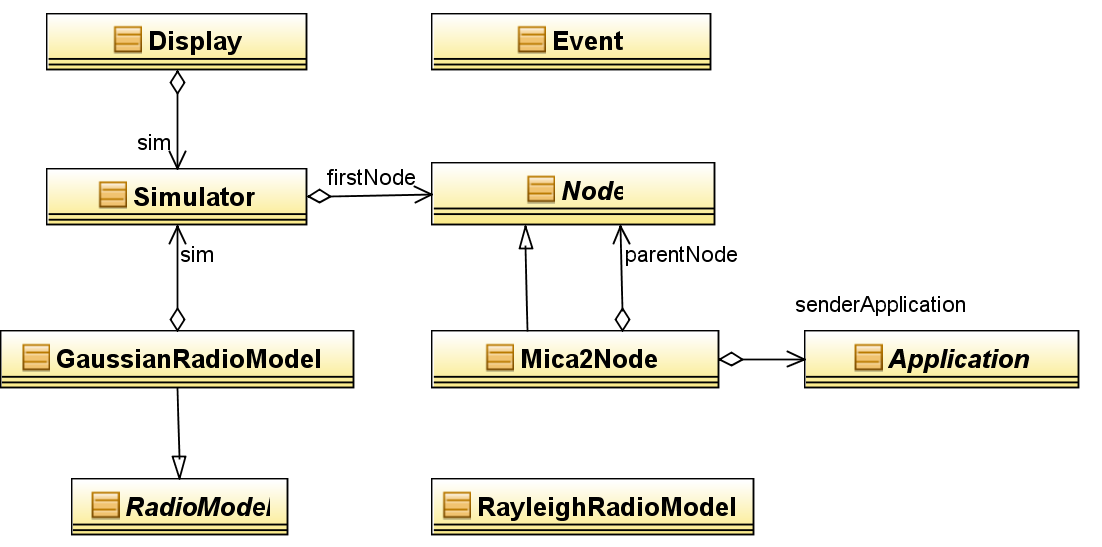
\includegraphics[height=4cm,width=10cm]{JProwlerClassDiagram.png}
\caption{Diagrama de classes do simulador JProwler}
\label{fig:jprowler_cd}
\end{figure}

O simulador base, JProwler\cite{jprowler}, � composto por um conjunto de nove
 classes que s�o representadas no diagrama \ref{fig:jprowler_cd}. Este simulador
est� estruturado em tr�s grupos de fun��es: a) Motor de simula��o, que
representando o ambiente de opera��o de uma RSSF, caracterizado pelo gerador de
eventos discretos e modelos de r�dio (Simulator, Event, RadioModel); b)
Plataformas de execu��o, que simulam o comportamento dos n�s sensores (Node,
Mica2Node, Application); c) Visualiza��o, permitindo observar a topologia da
rede. 

Para utilizar este simulador no estudo de um protocolo de encaminhamento,
tal como existe actualmente, � necess�rio implementar uma classe derivada de
Application com a l�gica do protocolo. A implementa��o de uma plataforma sensor,
disponibilizada no JProwler\cite{jprowler}, � monol�tica ou seja n�o observa uma
divis�o por camadas, como a apresentada em \cite{VERCITACAODAPILHA}. � certo
que nas plataformas f�sicas observa-se uma forte afinidade entre as camadas do
sensor, uma vez que algumas vezes ao n�vel aplica��o � necess�rio ter acesso a
dados da camada MAC ou transporte, de modo a facilitar o controlo do estado da
aplica��o, por exemplo, para a implementa��o de alguma forma de fiabilidade por
retransmiss�o. 

Este simulador n�o incorpora algumas das funcionalidades que se consideram 
interessantes de observar, de forma gen�rica, quando se pretende avaliar um
protocolo de encaminhamento seguro em RSSF. Um exemplo � a capacidade de ter uma
vis�o do consumo de energia da rede durante uma simula��o e poder observar o seu
impacte durante a opera��o e quando esta rede est� sujeita a um qualquer
ataque dos j� estudados. 

\subsection[Funcionamento do simulador JProwler]{Funcionamento do simulador
JProwler} 
Como j� foi referido o simulador procura ir ao encontro do funcionamento dos 
\textit  {motes} Mica2\cite{mica2_datasheet}  e com o sistema de eventos
implementado pelo TinyOS\cite{tinyos}. Neste sistema em cada momento apenas est�
a ser tratada uma mensagem de cada vez, o que faz com que,  caso cheguem v�rias
mensagens ao mesmo tempo, algumas mensagens se possam perder. O modelo de r�dio
preconiza um mecanismo de \textit{backoff} em caso de falha na transmiss�o. A
introdu��o de ru�do na transmiss�o � materializada com base numa distribui��o de
Gauss, este ru�do permite aproximar do comportamento de uma rede real. A
exist�ncia de uma pilha de eventos que executa um conjunto de eventos em cada
itera��o permite simular a ocorr�ncia de diversos eventos em diferentes pontos
da rede, ao mesmo tempo. Considerando, no entanto, que a no��o de tempo �
intr�nseca ao simulador, e que assim sendo um conjunto de eventos ocorre ao
mesmo tempo, em tempo de simula��o. 

A interface gr�fica disponibilizada, apenas permite a visualiza��o dos n�s 
sensores e a obten��o de alguma informa��o referente ao estado da transmiss�o,
materializada por um c�digo de cores, a possibilidade de dispor um determinado
n� sensor de forma orientada com recurso a um sistema \textit{drag-and-drop} n�o
se encontra dispon�vel. A distribui��o dos n�s na �rea de trabalho � realizado
de forma aleat�ria, permitindo obter uma rede com alguma homogeneidade no que
respeita � distribui��o dos sensores pela �rea. A implementa��o dos sensores,
n�o preconiza a exist�ncia de diversos estados de opera��o dos sensores, ou
seja, � semelhan�a do que se observa ao n�vel da gest�o de energia de um sensor
durante o seu ciclo de vida, com os estados, por exemplo, activo, inactivo e
adormecido. Estes estados s�o, normalmente, geridos ao n�vel MAC dependendo dos
protocolos que cada sensor implementa\cite{SMAC, BMAC}.
INCLUIR IMAGEM DO JPROWLER GUI
\section{Proposta para a arquitectura da plataforma de simula��o}
\label{sec:apresent_arch}

Para melhor percep��o da arquitectura da plataforma de simula��o, esta � 
apresentada sob a  forma de uma pilha de servi�os. Como se
pode ver na \figurename{ \ref{fig:sim_arch}}, os principais servi�os s�o: 
i) Simulador base ou motor de simula��o; ii) Camada de Instrumenta��o e Teste;
iii) API para a implementa��o e avalia��o de protocolos de encaminhamento; iv)
Consola de visualiza��o e controlo de simula��o.
\begin{figure}[ht]
\centering
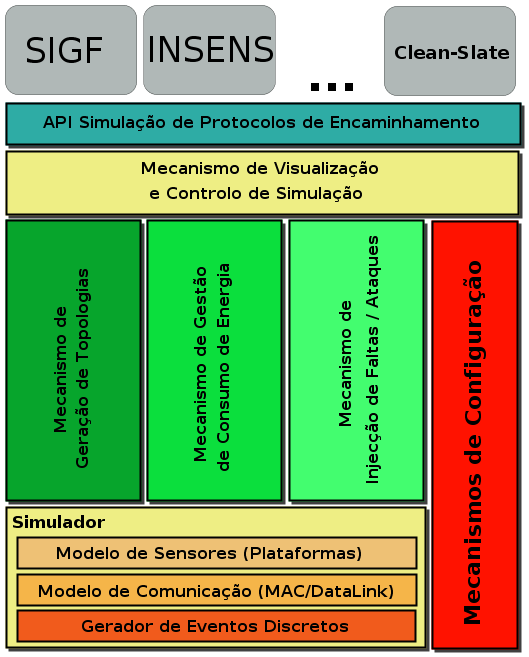
\includegraphics[height=9cm,width=8cm]{Simulador_arquitectura.png}
\caption{Arquitectura de Simula��o} \label{fig:sim_arch}
\end{figure}
\subsection[Simulador base ou motor de simula��o]{Simulador base ou motor de
simula��o}
Como j� foi referido o motor de simula��o resulta da extens�o do simulador 
JProwler. De uma forma geral, o simulador j� implementa os modelos base de um
RSSF, nomeadamente no que respeita ao modelo de acesso ao meio e no modelo
r�dio. 
\subsection[Camada de instrumenta��o]{Camada de instrumenta��o}
Esta camada cont�m um conjunto de ferramentas que controlam a simula��o 
nomeadamente no que respeita aos mecanismos principais que se pretendeu
implementar na plataforma: 
\subsubsection{Mecanismo de Configura��o}\label{sec:impl_conf}
Para dotar a plataforma de maior flexibilidade, a exist�ncia de um componente
 gestor de configura��es revela-se importante. Este componente deve ser
transversal a toda 
plataforma. Para que as parametriza��es possam ser persistentes e port�veis, 
adoptar-se-� a tecnologia XML para a defini��o dos ficheiros de configura��o da
plataforma. As principais funcionalidades que se prev�em existir v�o desde as
configura��es dos par�metros do simulador base, at� � configura��o de cada uma
das simula��es que se pretendem estudar, como forma de possibilitar a repeti��o
de experi�ncias nas mesmas condi��es.
\subsubsection{Mecanismo de Gera��o de Topologias}\label{sec:impl_topo}
As RSSF, normalmente, s�o caracterizadas por diferentes formas de distribui��o
dos n�s sensores. Estas distribui��es podem ser essencialmente divididas em dois modelos:
aleat�rio e estruturado. Assim, para que se consiga observar as
caracter�sticas que se pretendem analisar num protocolo de encaminhamento, �
fornecido um componente cuja fun��o � gerar topologias na rede. Sabe-se que, de facto, a
topologia da rede pode influenciar o comportamento de um protocolo. Pretende-se que este
componente possibilite a extens�o para novas topologias (espec�ficas para determinada
simula��o).
\subsubsection{Mecanismos de medi��o de propriedades
da rede}\label{sec:impl_energia}
Por forma a permitir a avalia��o de protocolos de encaminhamento foi necess�rio
 proceder-se ao desenvolvimento de ferramentas de medi��o de propriedades que se
pretendia observar em cada um dos protocolos. A energia, a cobertura da rede, a
lat�ncia das comunica��es e a fiabilidade da rede s�o as propriedades principais
que necessitaram de ver implementados componentes espec�ficos para avalia��o em
cada simula��o ou experi�ncia.
\paragraph{M�dulo de Energia}
Este � um dos componentes de maior import�ncia, uma vez que um dos
indicadores que se pretende observar na an�lise de protocolos de encaminhamento 
� o impacte sobre o tempo �til de opera��o da rede, quer em condi��es de
funcionamento normais, quer  em condi��es de ataque efectivo, tempo este que
est� dependente da energia. 
A energia � um recurso escasso numa RSSF. Para a implementa��o de mecanismos de 
seguran�a, � necess�rio recorrer a maior computa��o, transmiss�o de dados de
forma segura e capacidade de verifica��o de determinadas propriedades de
seguran�a. Sendo reconhecida a import�ncia desta ferramenta os princ�pios
orientadores para a sua implementa��o foram: i) Tornar a expressividade destes
consumos na l�gica dos protocolos o mais transparente poss�vel; ii) Adoptar um
modelo o mais pr�ximo poss�vel da realidade, principalmente no que refere aos
consumos de cada opera��o de um n� sensor; iii) Parametriza��o do modelo de
energia por forma a permitir a calibra��o o mais pr�xima do valores reais; iv)
Capacidade para analisar em p�s processamento os dados resultantes da an�lise de
consumo energ�tico, para a elabora��o de gr�ficos representativos dos resultados
obtidos; v) Capacidade de, em tempo real, prever os perfis de consumo de modo a
evitar a execu��o de longas simula��es sem que os resultados obtidos se revelem
desnecess�rios para o estudo em causa.

\paragraph[]{M�dulo de Cobertura/Fiabilidade/Lat�ncia da Rede}
Mediante as tipologias de ataques estudadas, observa-se que, um dos resultados 
destes ataques � a possibilidade de criar parti��es numa rede, limitar as
comunica��es de modo selectivo ou alterar de modo total ou parcial a informa��o
de encaminhamento resultando, em qualquer um dos casos, na perda de dados.
Assim, interessa desde logo observar a capacidade de resist�ncia de um protocolo
quando sujeito a determinados ataques e aferir com isto qual o n�vel de
disponibilidade da rede durante estas fases. N�o obstante este facto, a rede
dever� sempre ser medida no seu funcionamento normal e n�o sujeito a ataques.
Com este m�dulo, � poss�vel medir as propriedades de cobertura, fiabilidade e
lat�ncia da rede segundo seguintes as defini��es:
\begin{description}
\item[Cobertura:] � entendida como a capacidade de um qualquer sensor da rede
conseguir comunicar com um qualquer outro n� da rede utilizando o protocolo de
encaminhamento de dados implementado. A an�lise resultante da observa��o desta
capacidade pode ser comparada com a cobertura estabelecida pela comunica��o
r�dio. Interessa portanto real�ar que apesar de todos os sensores de uma rede
estarem cobertos em certa medida, por comunica��o r�dio, isso n�o � condi��o
suficiente para para garantir a transmiss�o de dados de um qualquer ponto A
para um qualquer ponto B, uma vez que podem existir parti��es na rede.

\item[Fiabilidade:] � entendida como a medida que avalia a qualidade da
comunica��o face ao modo de transmiss�o, modo este que compreende toda a camada
de software utilizada na arquitectura de um sensor. Assim, o resultado da
an�lise desta medida indica o �ndice de qualidade de informa��o  que um
qualquer sensor pode enviar para outro. � medida tendo em conta o numero de
mensagens enviadas face �s mensagens recebidas entre quaisquer dois sensores
de uma rede, tipicamente um sensor gerador de eventos e uma esta��o base.
Alguns par�metros podem ainda afectar os resultados observados, como por
exemplo o n�mero de retransmiss�es de cada mensagem e o intervalo de tempo
entre o envio de cada mensagem, que, quando mal parametrizados podem contribuir
para a perda de qualidade de comunica��o na rede.

\item[Lat�ncia:] Tratando-se de redes, a lat�ncia � uma m�trica
sempre a ter presente na sua analise. Esta medida pode ser efectuada
de duas formas: a) por tempo decorrido no envio de mensagens entre dois pontos;
b) por numero de n�s percorridos no envio de mensagens entre dois pontos. A
primeira pode ser dif�cil de medir, uma vez que se trata de um sistema simulado,
em que o factor tempo nem sempre tem a resolu��o que permite aferir com
rigor a qualidade desta medida. No segundo caso, o n�mero de \textit{hops}
percorridos por uma mensagem pode ser uma medida bastante gen�rica e precisa que
permite aferir esta propriedade da comunica��o entre dois quaisquer pontos,
podendo-se depois deste modo extrapolar um valor estimado para o tempo decorrido
em fun��o de uma largura de banda especificada. No entanto, se se pretender
avaliar a possibilidade de utiliza��o de um protocolo em aplica��es em que o
tempo de resposta � central, torna-se tamb�m importante considerar o tempo como
unidade de medida a avaliar.
\end{description}

\subsubsection{Mecanismo de Injec��o de Falhas /Ataques}
\label{sec:impl_ataques}
A implementa��o deste componente reveste-se de grande import�ncia, para tal
dever� se ter em aten��o os seguintes pontos:
i) N�o existe nenhum sistema de simula��o que permita a indu��o de ataques de
forma simples e intuitiva, consubstanciado-se, por isso, num contributo para a
inova��o; ii) Dever� ser suficientemente flex�vel para se adaptar � l�gica de
cada algoritmo; iii) Poder� permitir a muta��o/visualiza��o do c�digo
malicioso em tempo de execu��o, por forma a perceber comportamentos 
dos protocolos face ao ataque;
iv) Idealmente dever� permitir acrescentar mais modelos de ataques, dos j�
tipificados neste relat�rio ou de outros que venham a ser identificados.

Com o mecanismo de injec��o de ataques procura-se tornar o mais intuitiva
poss�vel a sua utiliza��o, assumindo desde logo que um ataque a um sensor
implica a altera��o/supress�o do conte�do de uma mensagem. Assim, � poss�vel
neste modelo activar o modo de ataque em cada um dos sensores bem como
seleccionar o ataque que se pretende observar, podendo coexistir com diversos
outros ataques implementados. No entanto, est� limitada a opera��o de
apenas um de cada vez em cada sensor. � poss�vel medir o impacte do ataque pelo
n�mero de mensagens que atravessam os n�s atacantes, bem como pela observa��o
das propriedades avaliadas pelo mecanismo descrito na sec��o anterior.

\subsubsection{Execu��o de testes e recolha de resultados}
A avalia��o de um protocolo de encaminhamento, preconiza a repeti��o de
baterias de testes e a varia��o de alguns par�metros como base
de compara��o de resultados e por forma a se poder observar tend�ncias e
comportamentos da rede. O modelo de execu��o de testes e recolha de resultados
segue um modelo que permite sistematizar a sua utiliza��o face a
diversas distribui��es de RSSF. 
Este componente do simulador � importante uma vez que
permite agilizar o estudo e concentrar nas experi�ncias
o foco da avalia��o de um protocolo de encaminhamento de dados. Assim sendo,
compreende-se como experi�ncia, uma simula��o com as seguintes propriedades:

\begin{enumerate}
\item Topologia bem definida (aleat�ria, em grelha ou estruturada);
\item Protocolo de encaminhamento;
\item Modelo de Energia parametrizado;
\item Bateria de testes;
\item Ataques ao n�vel do encaminhamento;
\end{enumerate}

Estas propriedades permitem sistematizar a avalia��o de um qualquer protocolo
de encaminhamento de dados seguro/ou n�o, vejamos: Para avaliar quaisquer
protocolos � poss�vel cruzar estas propriedades de diversas formas e comparar os
resultados com uma abordagem met�dica. O que se observa em alguns
simuladores � que a forma de implementa��o dos testes � diferente em cada
protocolo o que pode levar a diferen�as que influenciem os resultados. Com a
defini��o destes crit�rios e da metodologia gen�rica de avalia��o de protocolos
� poss�vel na realidade ter a mesma base de compara��o para protocolos
diferentes, permitindo afinar as conclus�es no que concerne ao seu comportamento
em termos de seguran�a e no impacte nas propriedades que se pretende observar.

\subsection{Consola de Visualiza��o e Controlo de
Simula��o}\label{sec:impl_visual}
Existe a necessidade de dotar a plataforma de uma consola de opera��o, que
permita interagir com o simulador de forma intuitiva e f�cil. Como tal, �
necess�rio implementar um componente para visualiza��o gr�fica de toda
a simula��o, bem como o controlo de par�metros de execu��o e configura��o.
Neste sentido, foi desenvolvido um ambiente gr�fico integrado, que permite a
configura��o da plataforma, a configura��o e visualiza��o das simula��es e a
extrac��o de resultados relacionados com as medidas que se pretendem avaliar,
tamb�m sob a forma de gr�ficos.
\subsection{API para implementa��o de protocolos de encaminhamento}
Uma vez que o ponto de partida da plataforma � uma simulador que respeita uma
API, com a integra��o de novas funcionalidades com caracter�sticas de 
avalia��o em diferentes camadas do \textit{software} das plataformas
sensoriais, surge um conjunto de interfaces que garantem a inter-opera��o entre
os protocolos e o simulador facilitando a medi��o das propriedades j� indicadas.
No cap�tulo seguinte � poss�vel observar alguns destes interfaces que tornam a
utiliza��o de algumas funcionalidades o mais transparente poss�vel por forma a
permitir o mesmo tipo de ac��es de avalia��o que contribuem para uma melhor
sistematiza��o da an�lise entre diversas implementa��es de protocolos.
\subsection{Metodologia de utiliza��o da plataforma}
Pretende-se com esta plataforma contribuir para uma metodologia de avalia��o de
protocolos de encaminhamento, principalmente, facilitando a compara��o de
diferentes protocolos. Assim, assumiu-se desde cedo a necessidade de
estabelecer um modelo de utiliza��o da plataforma, modelo este que n�o �
obrigat�rio para a realiza��o de avalia��es com esta ferramenta sendo no
entanto o utilizado na prova de conceito e tendo-se constatado que facilita a
uma iterativa de an�lise com vista a melhorar/refinar os resultados obtidos.
Esta metodologia tem tr�s fases seguintes que ser�o descritas sumariamente de
seguida sendo que a segunda e terceira fase podem ser feitas uma vez e usadas
em diferentes protocolos estabelecendo-se logo como uma base de compara��o
para outros protocolos que se pretenda estudar.
\subsubsection{Implementa��o de protocolo}
Esta fase compreende a implementa��o da especifica��o do protocolo em estudo. A
utiliza��o das facilidades disponibilizadas pela API e o cumprimento dos
interfaces requeridos para a instrumenta��o do simulador representam as �nicas
obrigatoriedades na implementa��o. Uma vez feito isto algumas funcionalidades
apresentam-se dispon�veis sem que o implementador tenha feito qualquer esfor�o
adicional, como � o caso, por exemplo, dos consumos energ�ticos de transmiss�o,
recep��o e mudan�a de estados dos sensor. No \chaptername{
\ref{cap:implementacao}} ser�o apresentados mais detalhes quanto a esta fase.
\subsubsection{Caracteriza��o do ambiente de simula��o}
A caracteriza��o do ambiente de simula��o, refere-se essencialmente ao ambiente
de opera��o que se pretende estudar. A defini��o de caracter�sticas de opera��o
como por exemplo: 1) alcance r�dio; 2) topologias de rede; 2) atenua��o
radio ambiental; 4) altitude do terreno; 5)   defini��o de n�s base e a sua
localiza��o; permite estabelecer um modelo de simula��o que persiste entre
diferentes experi�ncias, retirando algum custo de configura��o e permitindo uma
abordagem incremental pela realiza��o de pequenos ajustes resultante da
observa��o de resultados ou de comportamentos n�o esperados.
\subsubsection{Execu��o/an�lise de testes e resultados}
%\subsubsection{Avalia��o da Solu��o}\label{sec:aval_solucao}
%Uma vez que a contribui��o efectiva para a componente de investiga��o de
%protocolos de encaminhamento seguros em RSSF ser� obtida com a concep��o de uma
%plataforma de
%simula��o que suporte o estudo e a an�lise desta problem�tica, importa
%sujeit�-la a uma avalia��o
%prim�ria que permita comprovar a sua utilidade e/ou identificar eventuais
%lacunas neste dom�nio.
%Assim, tendo esta avalia��o em vista, pretende-se contribuir com o estudo dos
%protocolos de
%encaminhamento seguro Clean-Slate e INSENS. Para isso, definem-se duas fases
%complementares na
%elabora��o da tese: uma que visa a implementa��o de um protocolo simples, que
%permita aferir o
%correcto funcionamento da plataforma, e outra que vise a implementa��o dos dois
%protocolos referidos,
%que ser�o alvo de uma an�lise comparativa com recurso �s funcionalidades da
%plataforma. 


\chapter[Plano de trabalho]{Plano de Elabora��o da Tese}
\label{cap:plano}
A elabora��o da tese realizar-se-� durante o 2� semestre de 2009/2010, iniciando a 22 de Fevereiro
de 2010. O plano apresentado estabelece cinco grandes actividades: an�lise, desenvolvimento,
prova de conceito, avalia��o e relat�rio, como se apresenta na \figurename{ \ref{fig:gantt}}.
\begin{figure}[H]
\centering
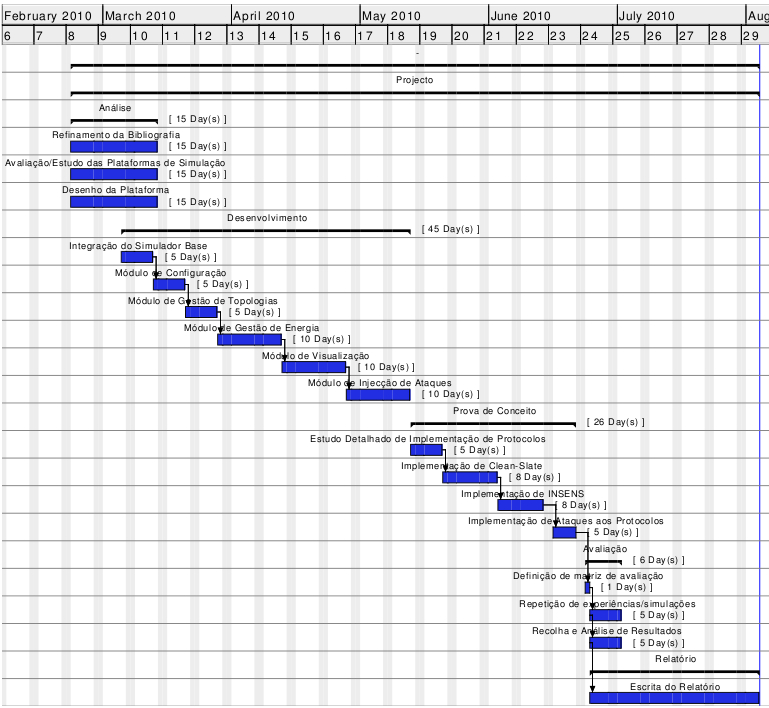
\includegraphics[height=16cm,width=18cm]{gantt.jpg}
\caption{Plano da Disserta��o} \label{fig:gantt}
\end{figure}
\newpage
Apresenta-se, em seguida, uma breve descri��o de cada uma das actividades.
\begin{description}
\item[An�lise]
Esta actividade corresponde � revis�o da bibliografia complementar, com um duplo objectivo: aprofundar a problem�tica em estudo e avaliar o simulador base, como preconizado na sec��o
\ref{sec:elab_aval_amb_sim}. Inicia-se, tamb�m, o desenho e a especifica��o da plataforma, consistindo na defini��o formal de algoritmos, de interfaces e do modelo de interac��o
dos componentes da plataforma. Durante a fase de desenvolvimento, esta actividade ser� revisitada,
com vista a refinar/actualizar a especifica��o da plataforma, nomeadamente pelo recurso a
ferramentas de modela��o de sistemas orientados a objectos (UML).
\item[Desenvolvimento]
Esta actividade corresponde � concep��o e implementa��o da arquitectura da plataforma, como
apresentada na sec��o \ref{sec:apresent_arch}, em que cada um dos componentes corresponder� �s
seguintes tarefas: Integra��o do Simulador Base, M�dulo de Configura��o (sec��o
\ref{sec:impl_conf}), M�dulo de Gest�o de Topologias (sec��o \ref{sec:impl_topo}), M�dulo de Gest�o
de
Energia (sec��o \ref{sec:impl_energia}), M�dulo de Visualiza��o (sec��o \ref{sec:impl_visual}) e
M�dulo de Injec��o de Ataques (sec��o \ref{sec:impl_ataques}).
\item[Prova de Conceito]
Esta actividade corresponde � implementa��o de um algoritmo b�sico ( ex: \textit{flooding} sem
repeti��o de mensagens enviadas) e  dos algoritmos de encaminhamento seguro
propostos (sec��o \ref{sec:impl_protocolos}): INSENS e Clean-Slate. Esta implementa��o dever�
ser precedida de um estudo mais aprofundado das particularidades de cada um. Consequentemente, cada
protocolo ser� sujeito a um modelo de ataque, que permitir� avaliar o seu comportamento, com vista a
verificar as propriedades, identificadas anteriormente como importantes, para a an�lise de um
protocolo de encaminhamento seguro em RSSF.
\item[Avalia��o]
Esta actividade preconiza a avalia��o dos protocolos implementados, usando as ferramentas da
plataforma, como referido na sec��o \ref{sec:aval_protocolos}. Esta avalia��o permitir�,
tamb�m, retirar conclus�es acerca da usabilidade da plataforma (sec��o \ref{sec:aval_solucao}) e dos objectivos pretendidos. Estes passam pela capacidade de estudo de
protocolos de encaminhamento em RSSF, em geral, e, em particular, os que t�m preocupa��es de seguran�a.
\item[Relat�rio]
Esta actividade corresponde � escrita da disserta��o e dever� iniciar-se assim que
termine o processo de especifica��o da plataforma, permitindo a realiza��o do modelo de
objectos. Esta fase poder� decorrer em paralelo com a actividade de avalia��o e, eventualmente, com a de prova de
conceito. Culminar� com a entrega da disserta��o at� � data limite.   
\end{description}


% ...
% \include{capituloN}

%% Parte ps-texto principal
\backmatter

% Apndices. Comente se no houver apndices
\appendix

%  aconselhvel ter um apndice por ficheiro
% "apendice1.tex", "apendice.tex", ... "apendiceM.tex" e depois
% inclu-los com:
% \include{apendice1}
% \include{apendice2}
% ...
% \include{apendiceM}

% Bibliografia. Deve utilizar o BibTeX a partir de um arquivo, ex: "mybib.bib".
\bibliographystyle{plain}
\bibliography{mybib}

%% Fim do documento
\end{document}
